\section{Evaluation des Précipitations}
\subsection{Evaluation Déterministe}
\begin{frame}{Précipitation}
\framesubtitle{Déterministe - ACC}

\begin{figure}
    \centering
    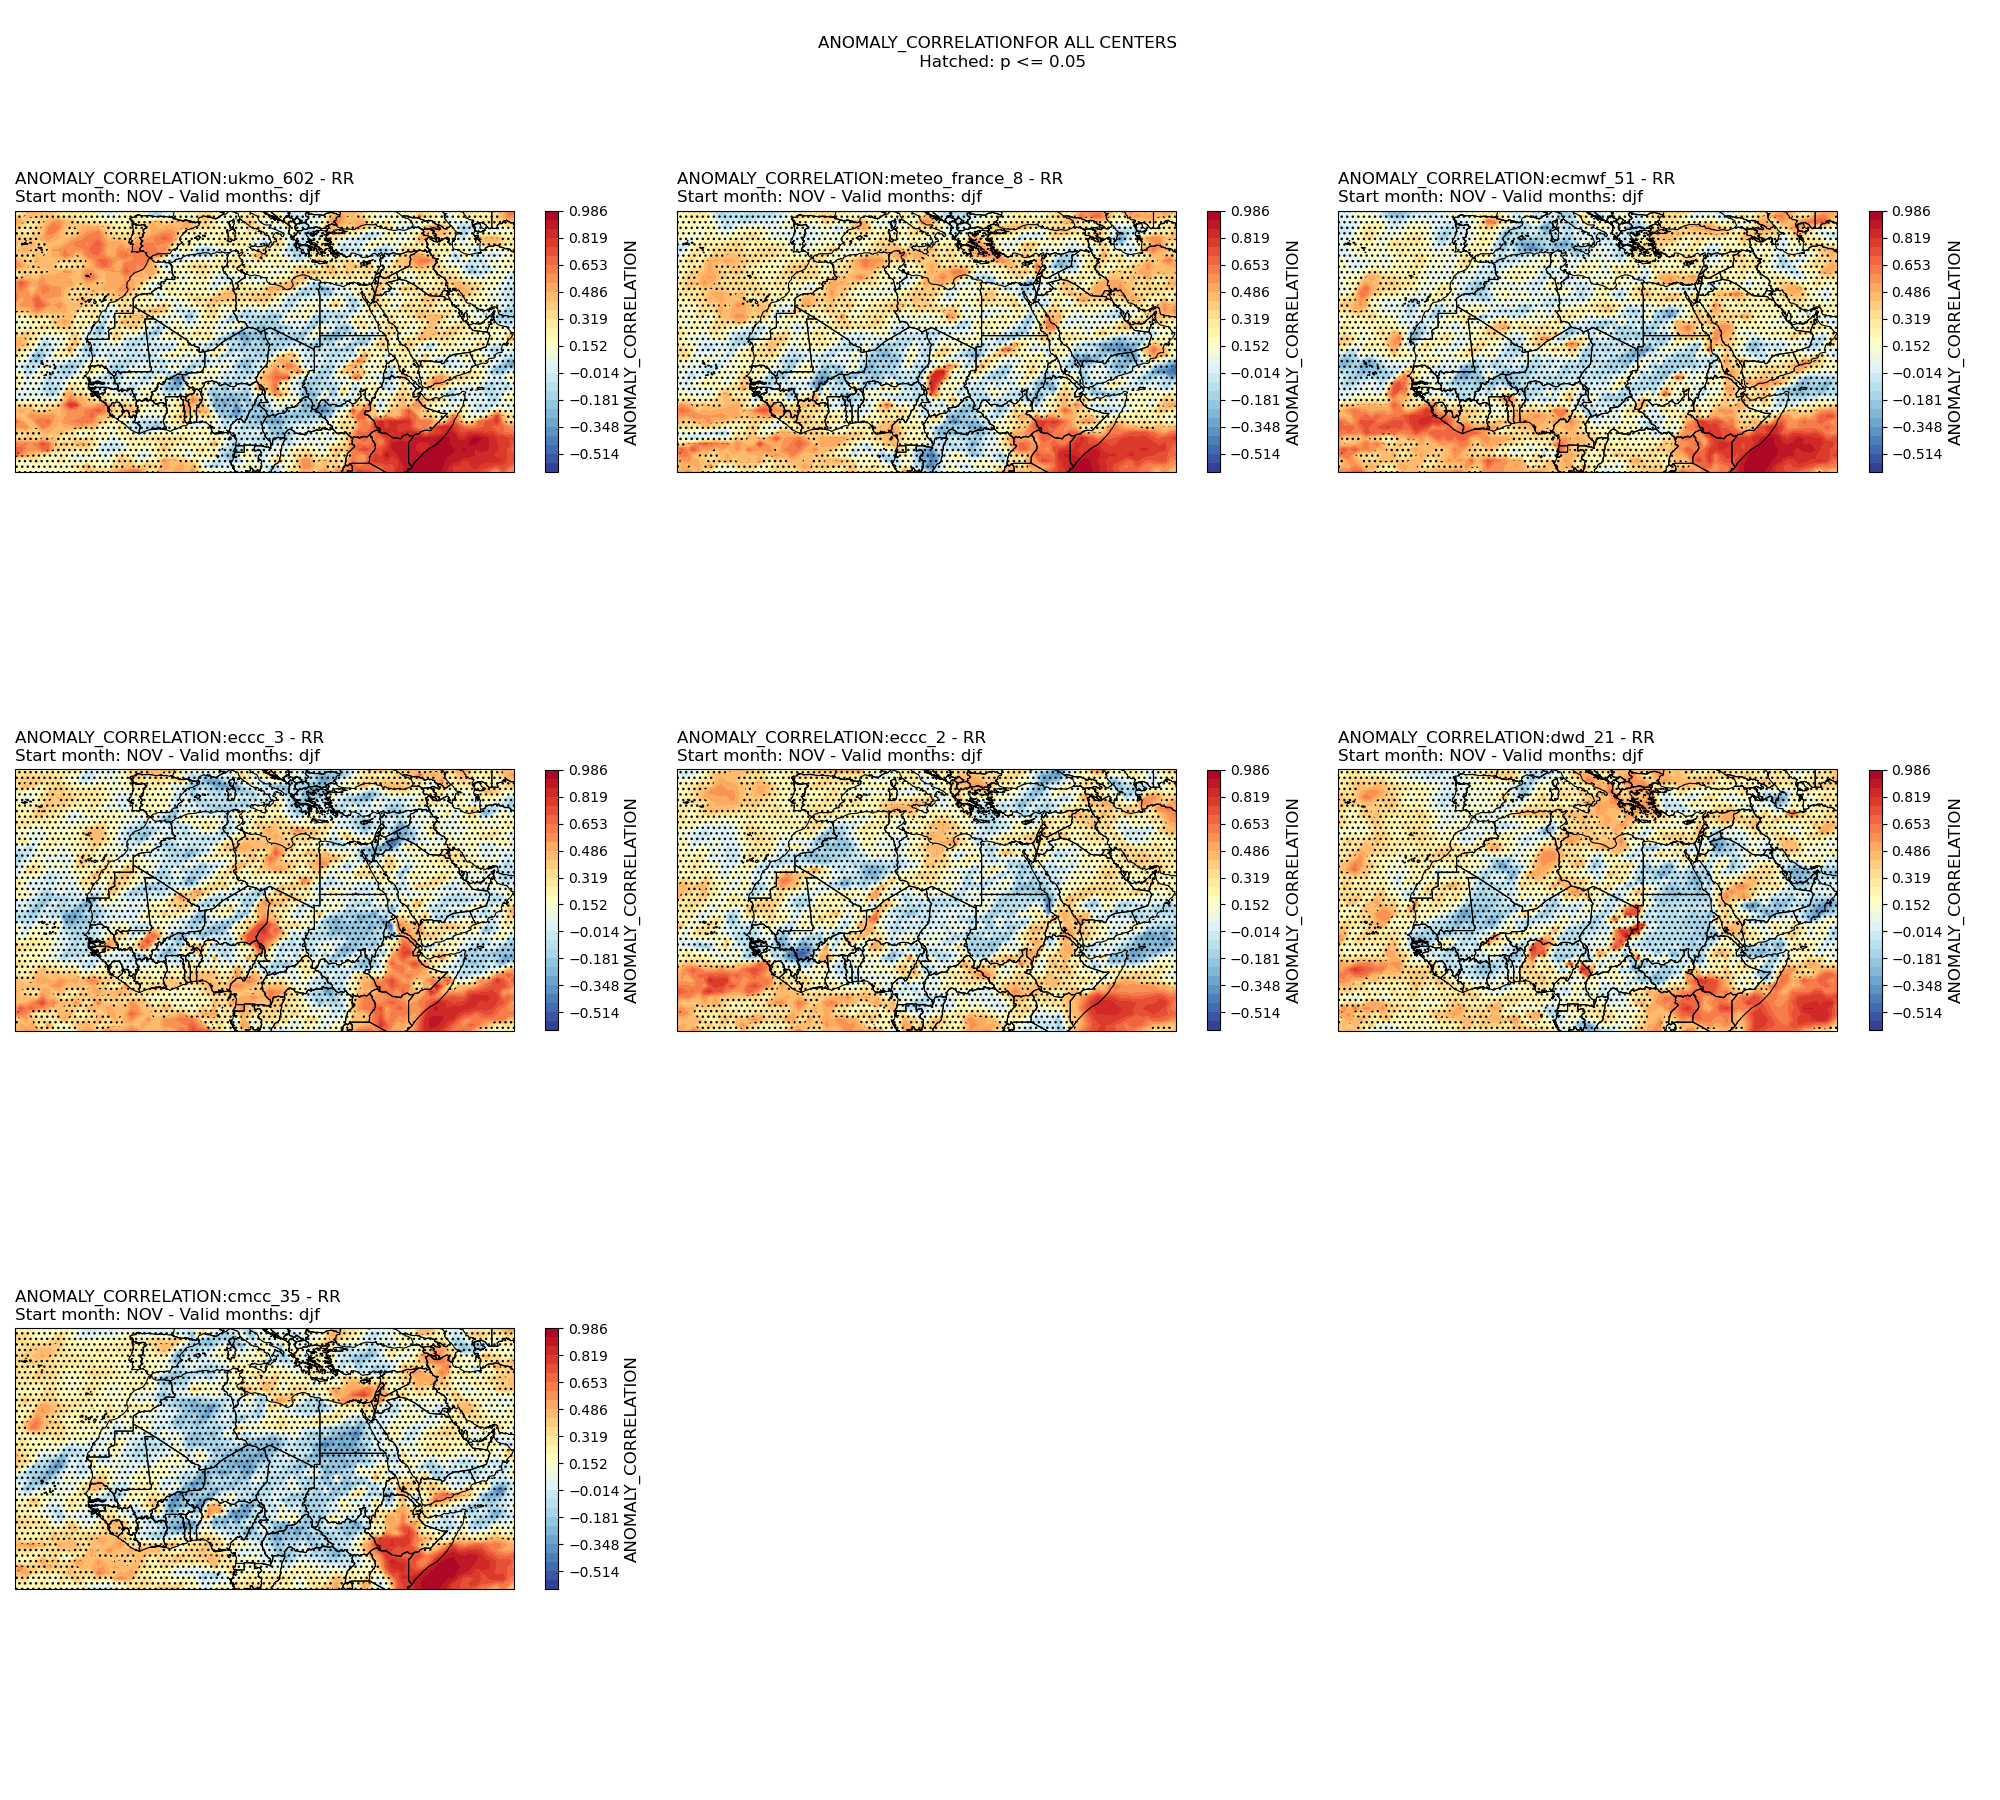
\includegraphics[width=0.7\linewidth]{/home/mohamed/EHTPIII/MODELISATION/Report_25_11/plots/det/acc/ANOMALY_CORRELATION_djf_RR.png}
    \caption{ACC pour les Precipitations - DJF  }
    \label{fig:enter-label}
\end{figure}
\end{frame}

\begin{frame}{Précipitation}
\framesubtitle{Déterministe - ACC}

\begin{figure}
    \centering
    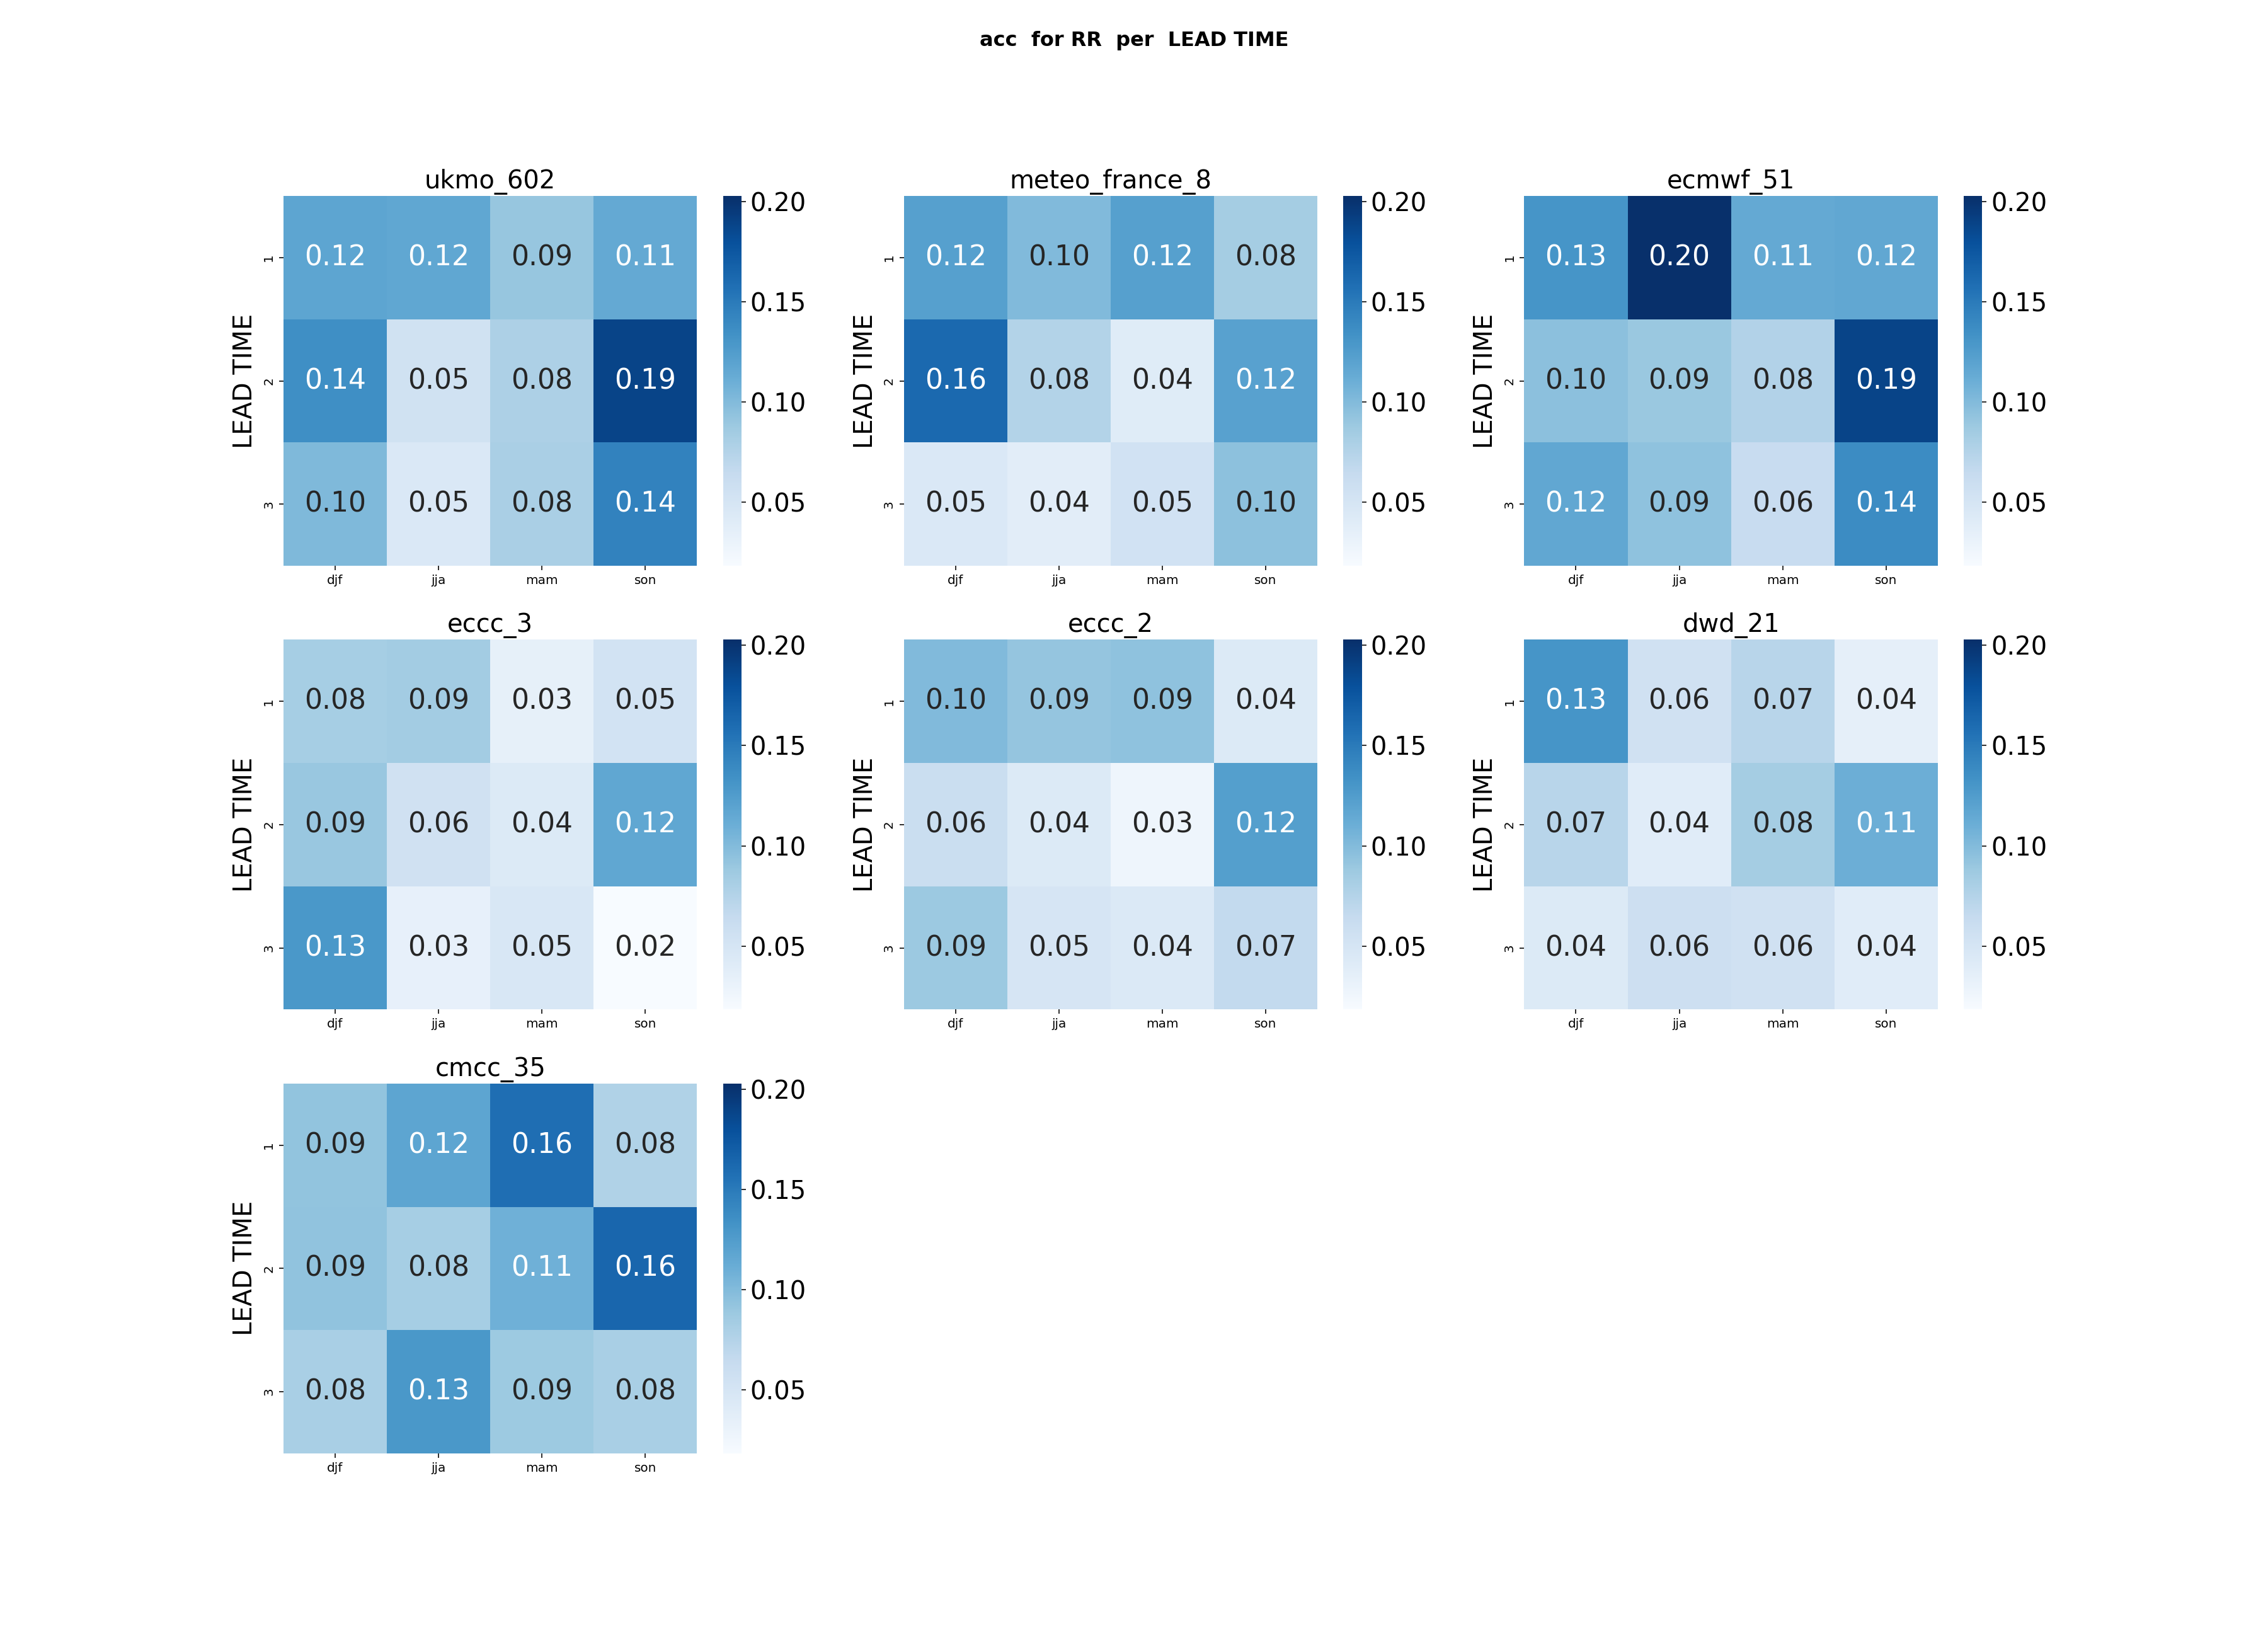
\includegraphics[width=0.8\linewidth]{/home/mohamed/EHTPIII/MODELISATION/Report_25_11/plots/det/acc/acc_RR_mena.png}
    \caption{Heatmap ACC pour les Precipitations  }
    \label{fig:enter-label}
\end{figure}
\end{frame}

\begin{frame}{Précipitation}
\framesubtitle{Déterministe - RMSE}

\begin{figure}
    \centering
    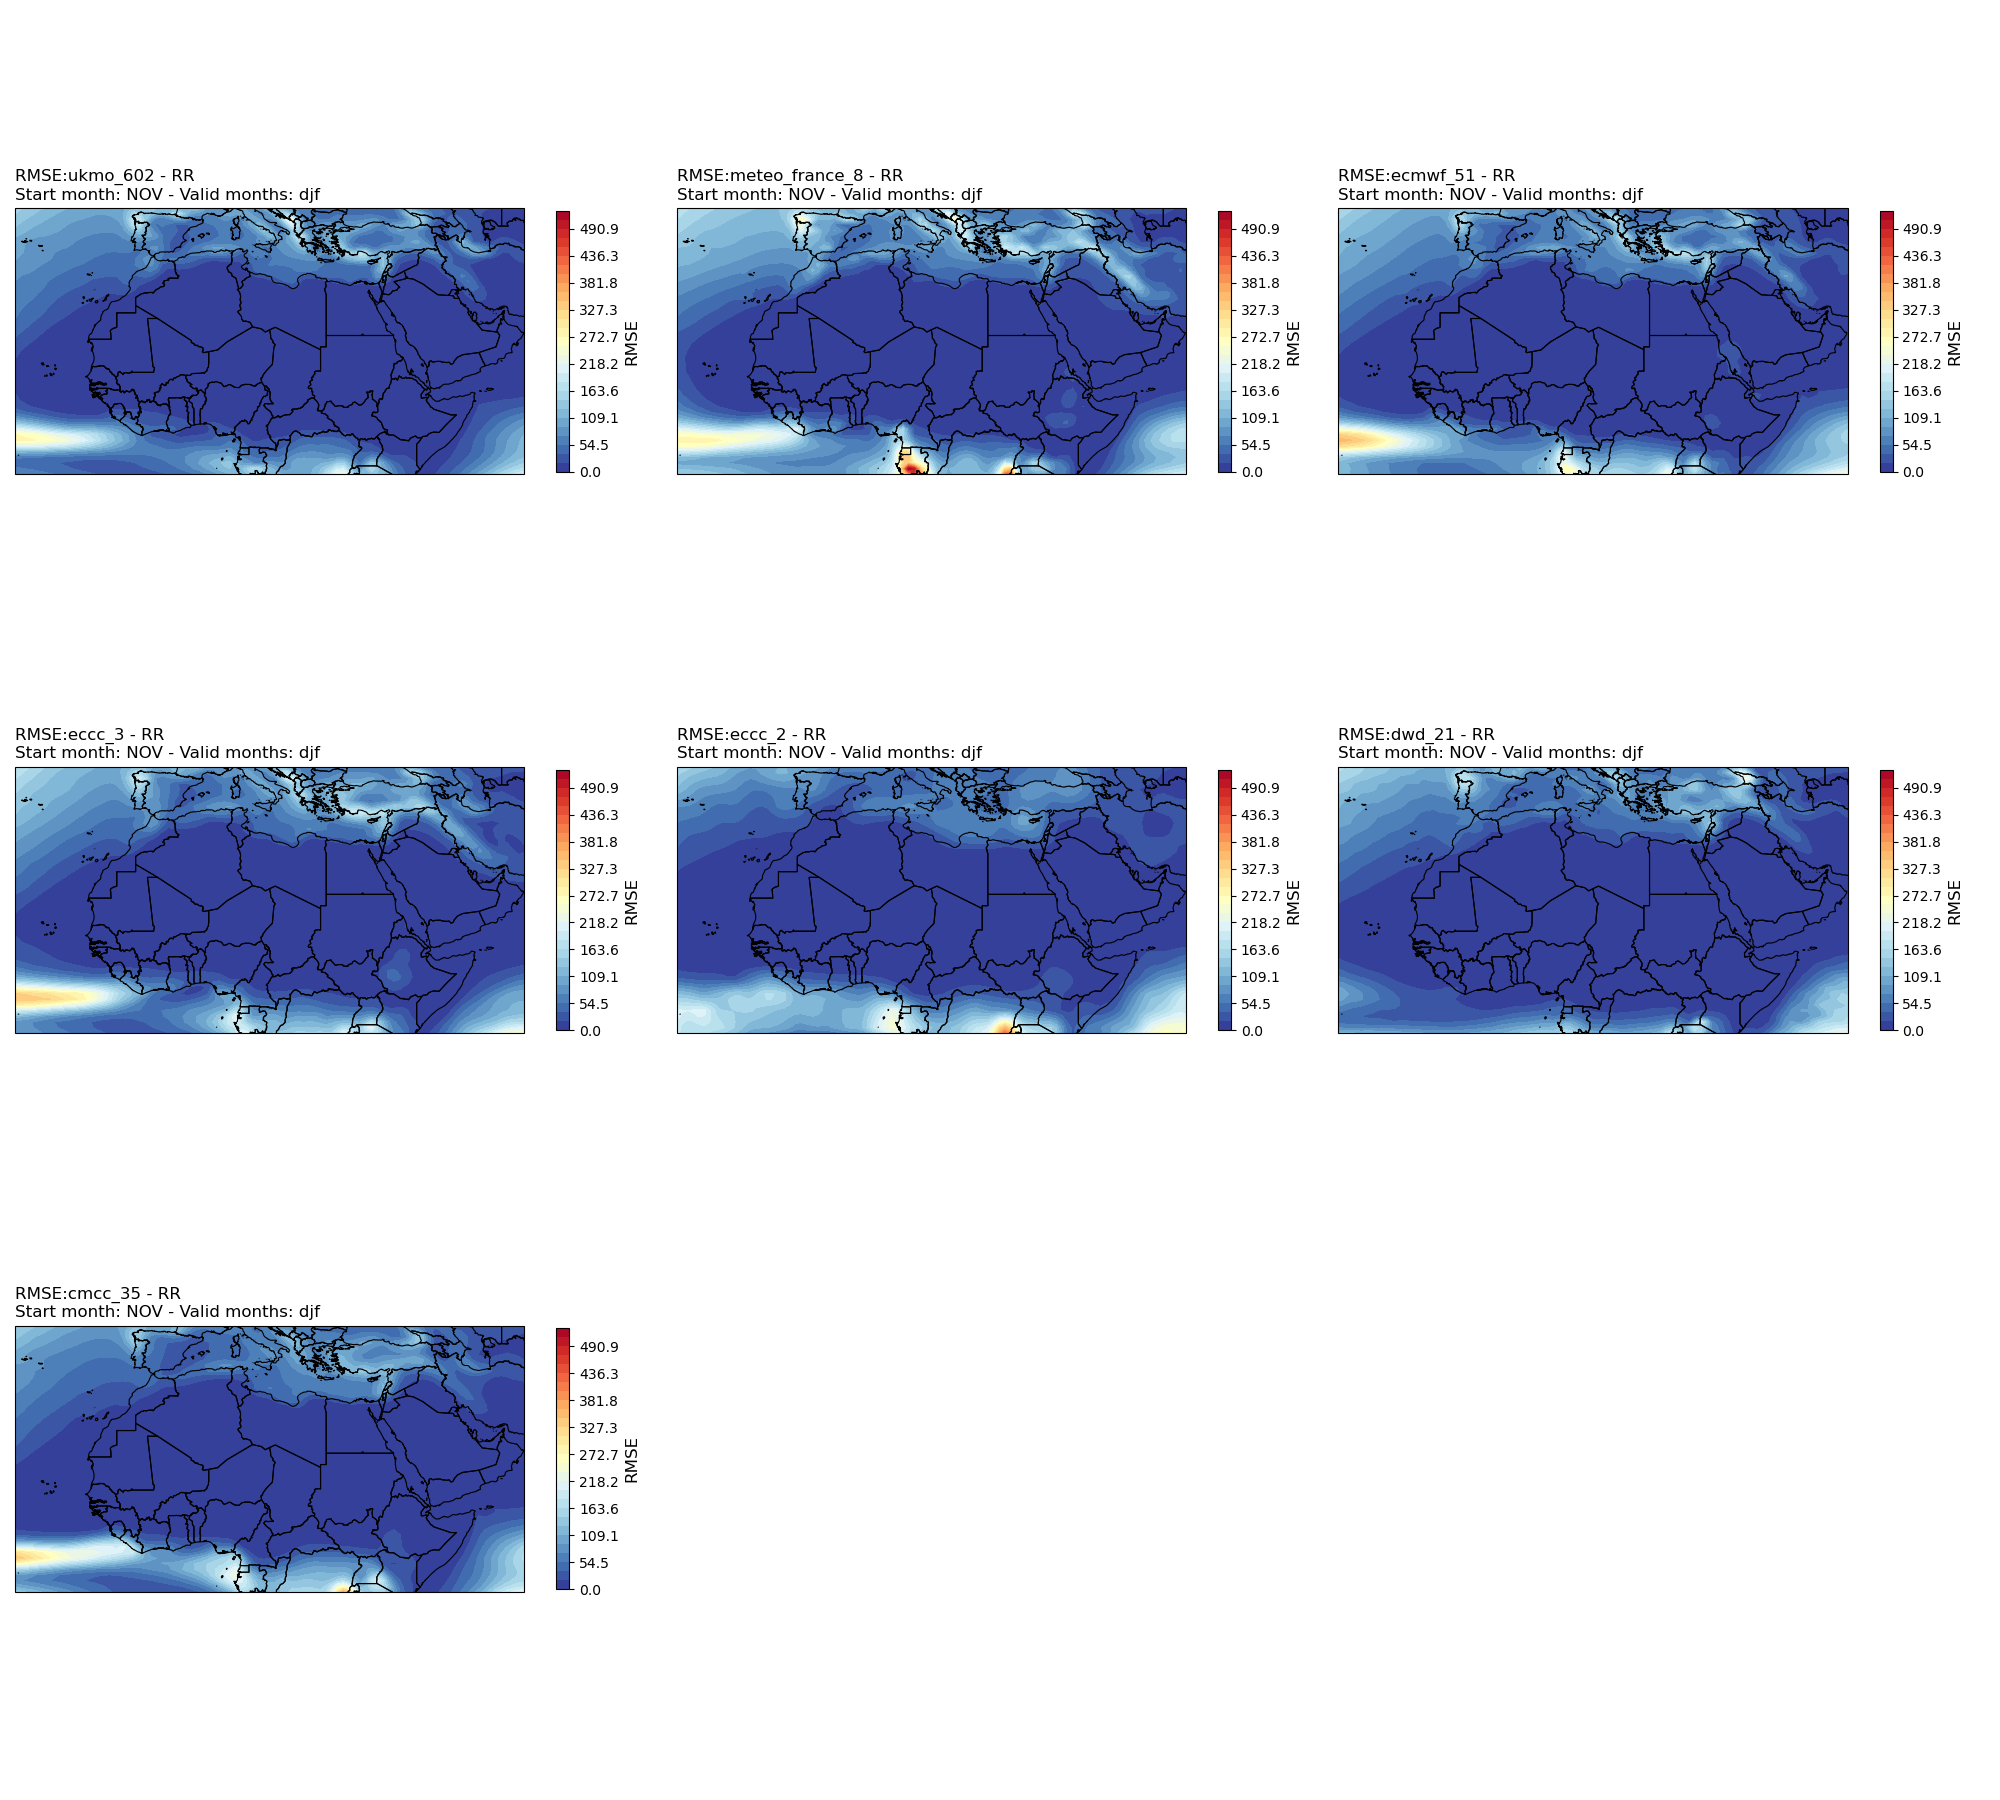
\includegraphics[width=0.7\linewidth]{/home/mohamed/EHTPIII/MODELISATION/Report_25_11/plots/det/rmse/rmse_djf_RR.png}
    \caption{RMSE pour les Precipitations - DJF  }
    \label{fig:enter-label}
\end{figure}
\end{frame}

\begin{frame}{Précipitation}
\framesubtitle{Déterministe - RMSE}

\begin{figure}
    \centering
    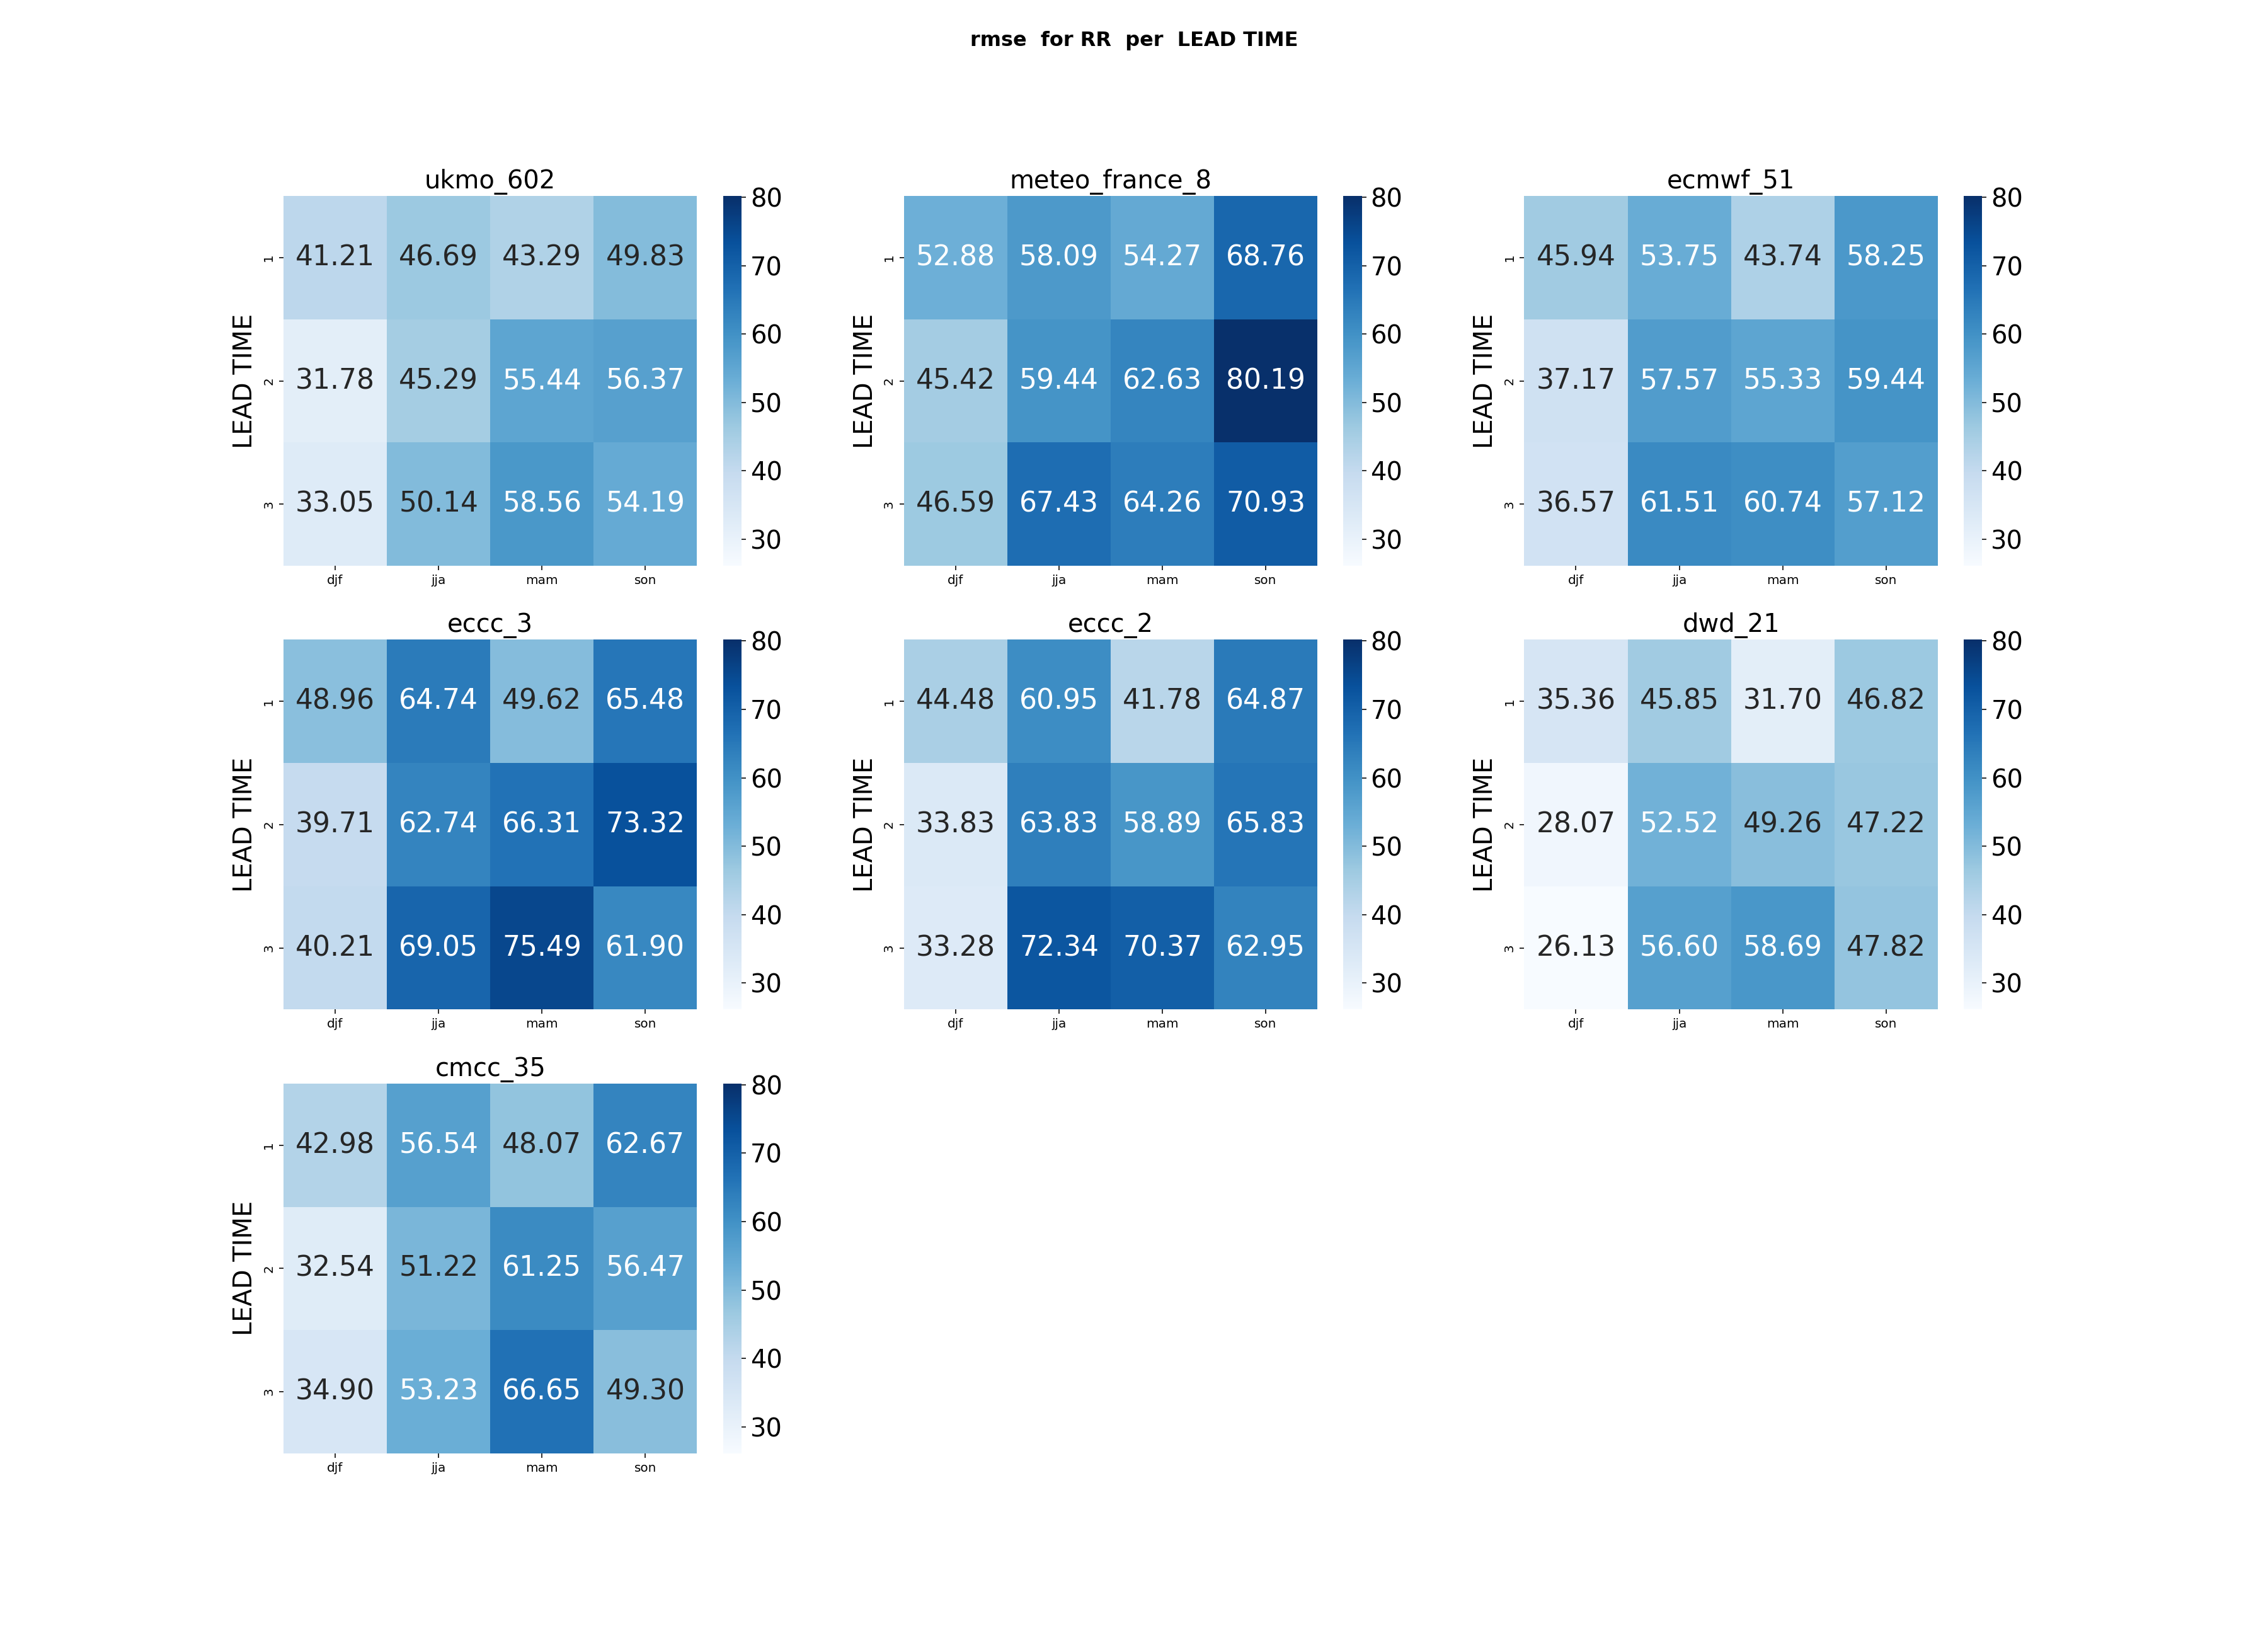
\includegraphics[width=0.8\linewidth]{/home/mohamed/EHTPIII/MODELISATION/Report_25_11/plots/det/rmse/rmse_RR_mena.png}
    \caption{Heatmap RMSE pour les Precipitations  }
    \label{fig:enter-label}
\end{figure}
\end{frame}

\subsection{Evaluation Probabiliste}

\begin{frame}{Précipitation}
\framesubtitle{Probabiliste - BS (0 pour un BS meilleur)}

\begin{figure}
    \centering
    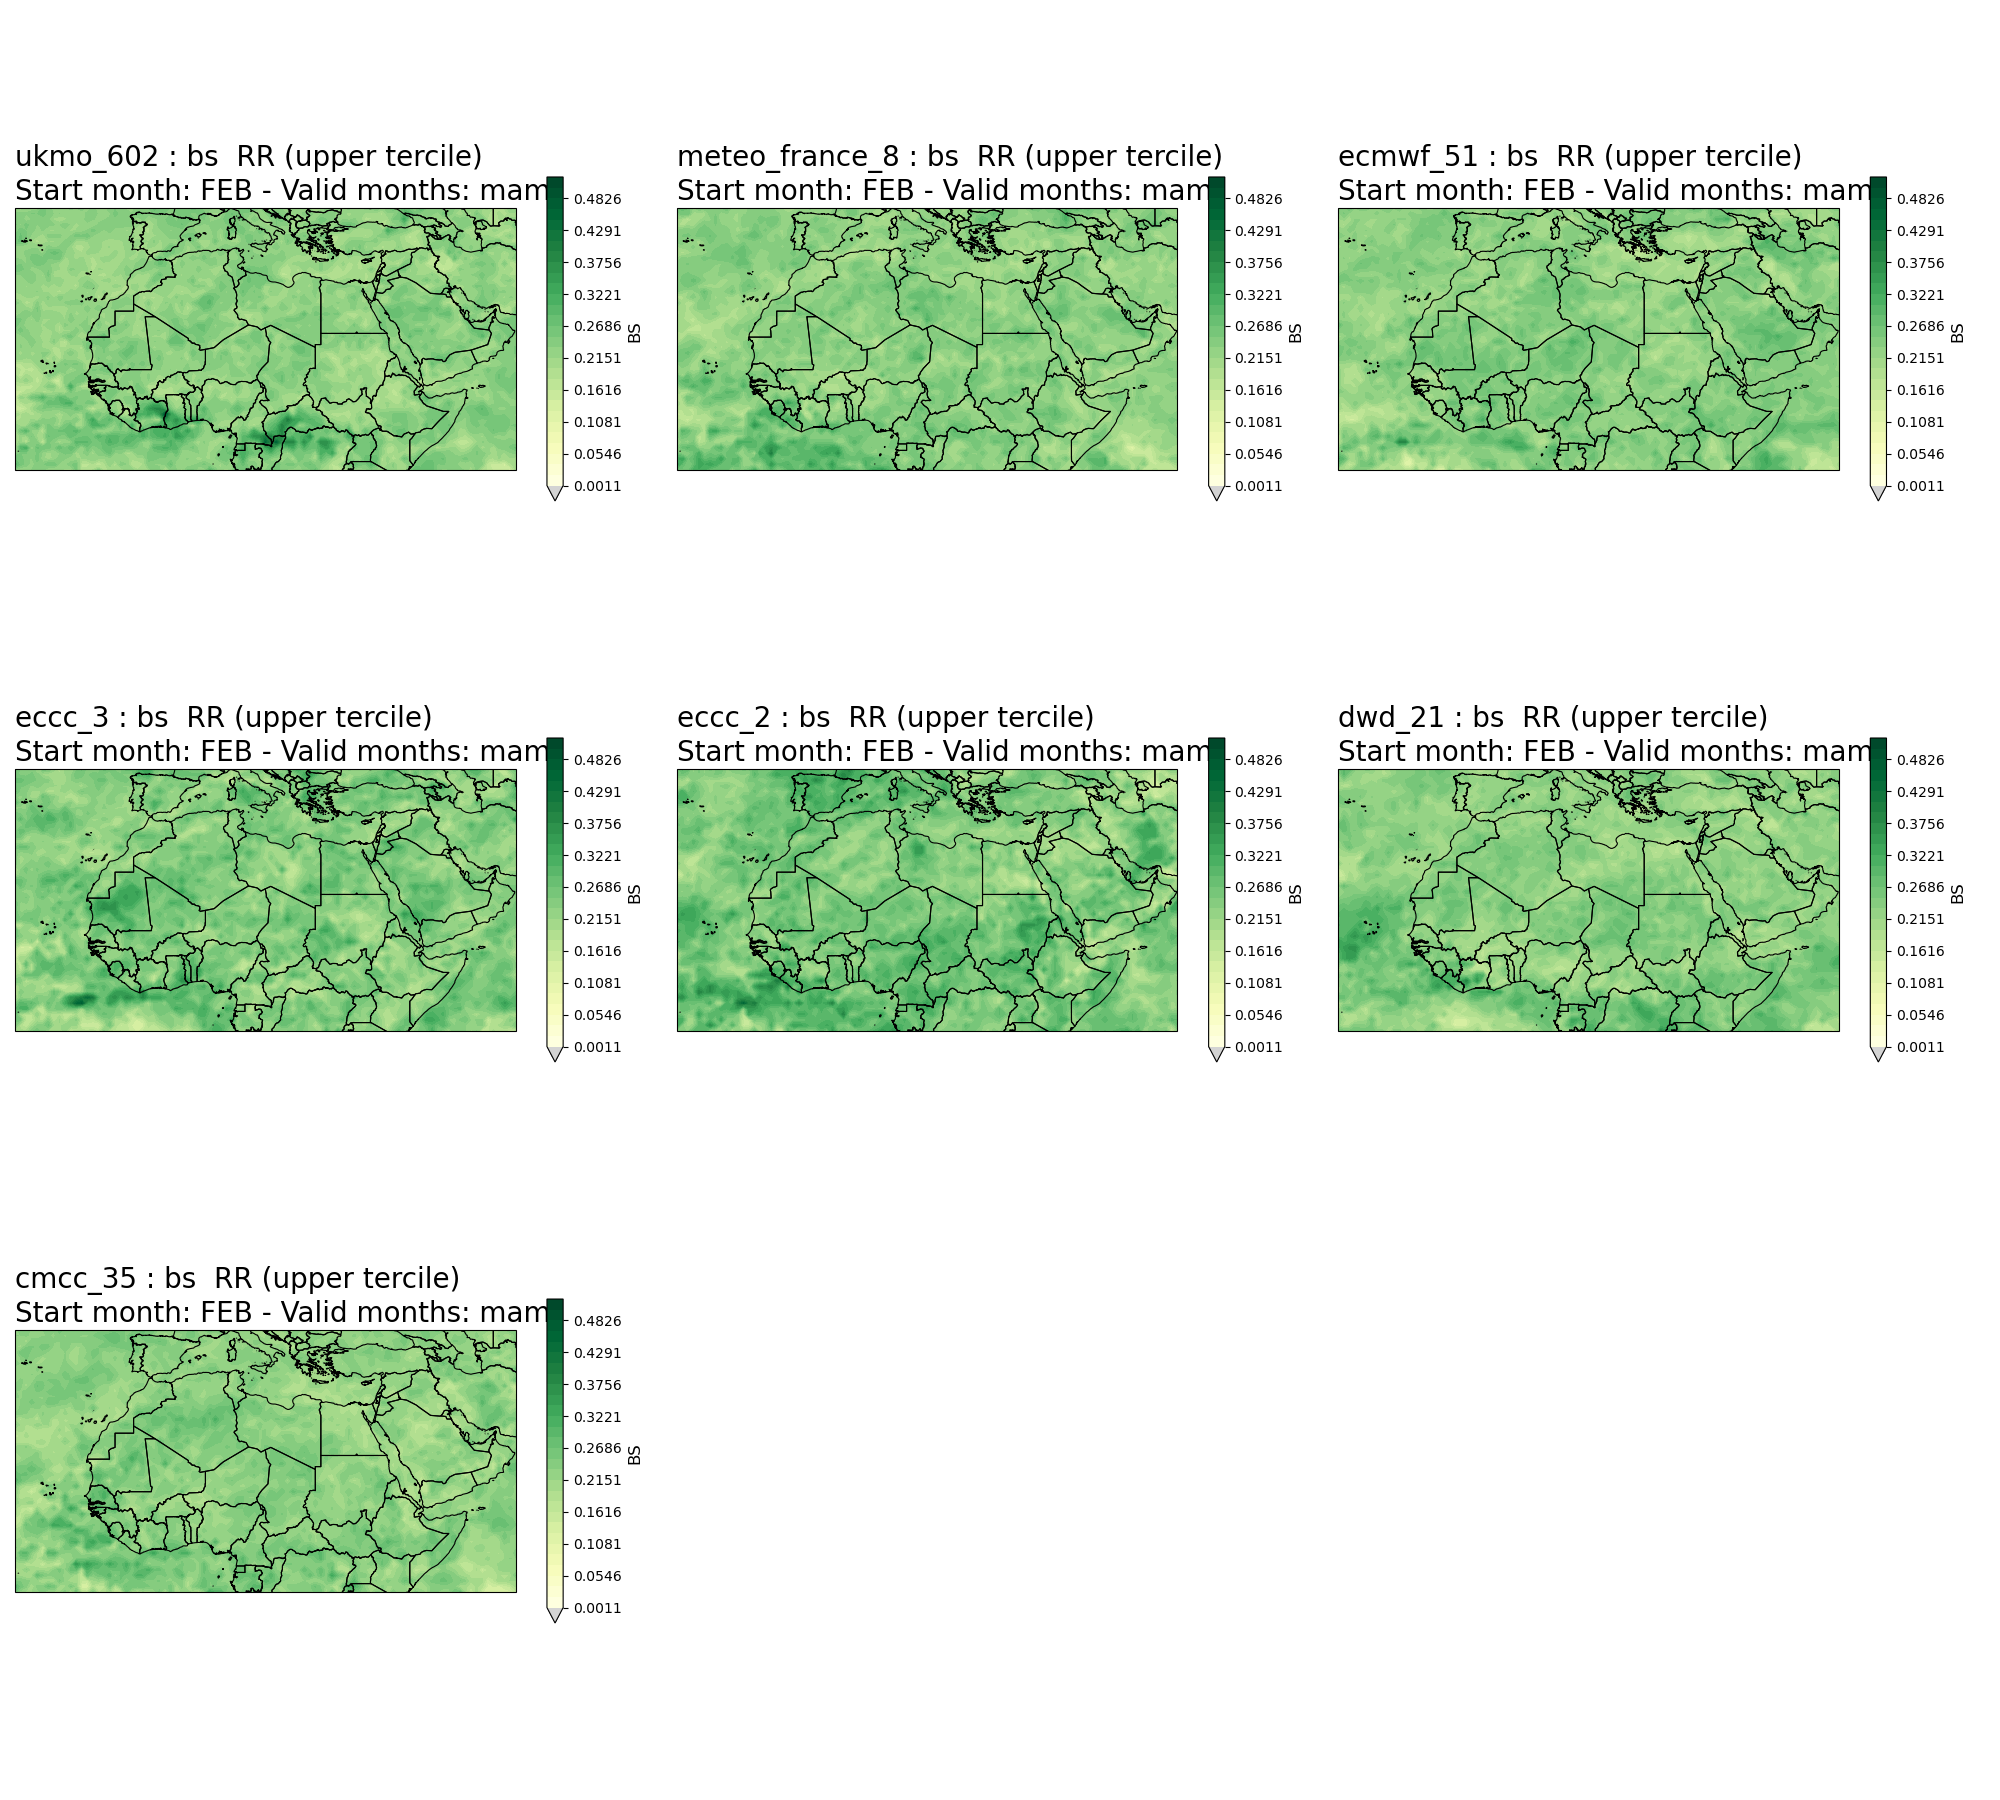
\includegraphics[width=0.7\linewidth]{/home/mohamed/EHTPIII/MODELISATION/Report_25_11/plots/prob/bs/bs_mam_upper_RR.png}
    \caption{BS pour les Precipitations - MAM  Upper Tercile }
    \label{fig:enter-label}
\end{figure}
\end{frame}

\begin{frame}{Précipitation}
\framesubtitle{Probabiliste - BS (0 pour un BS meilleur)}

\begin{figure}
    \centering
    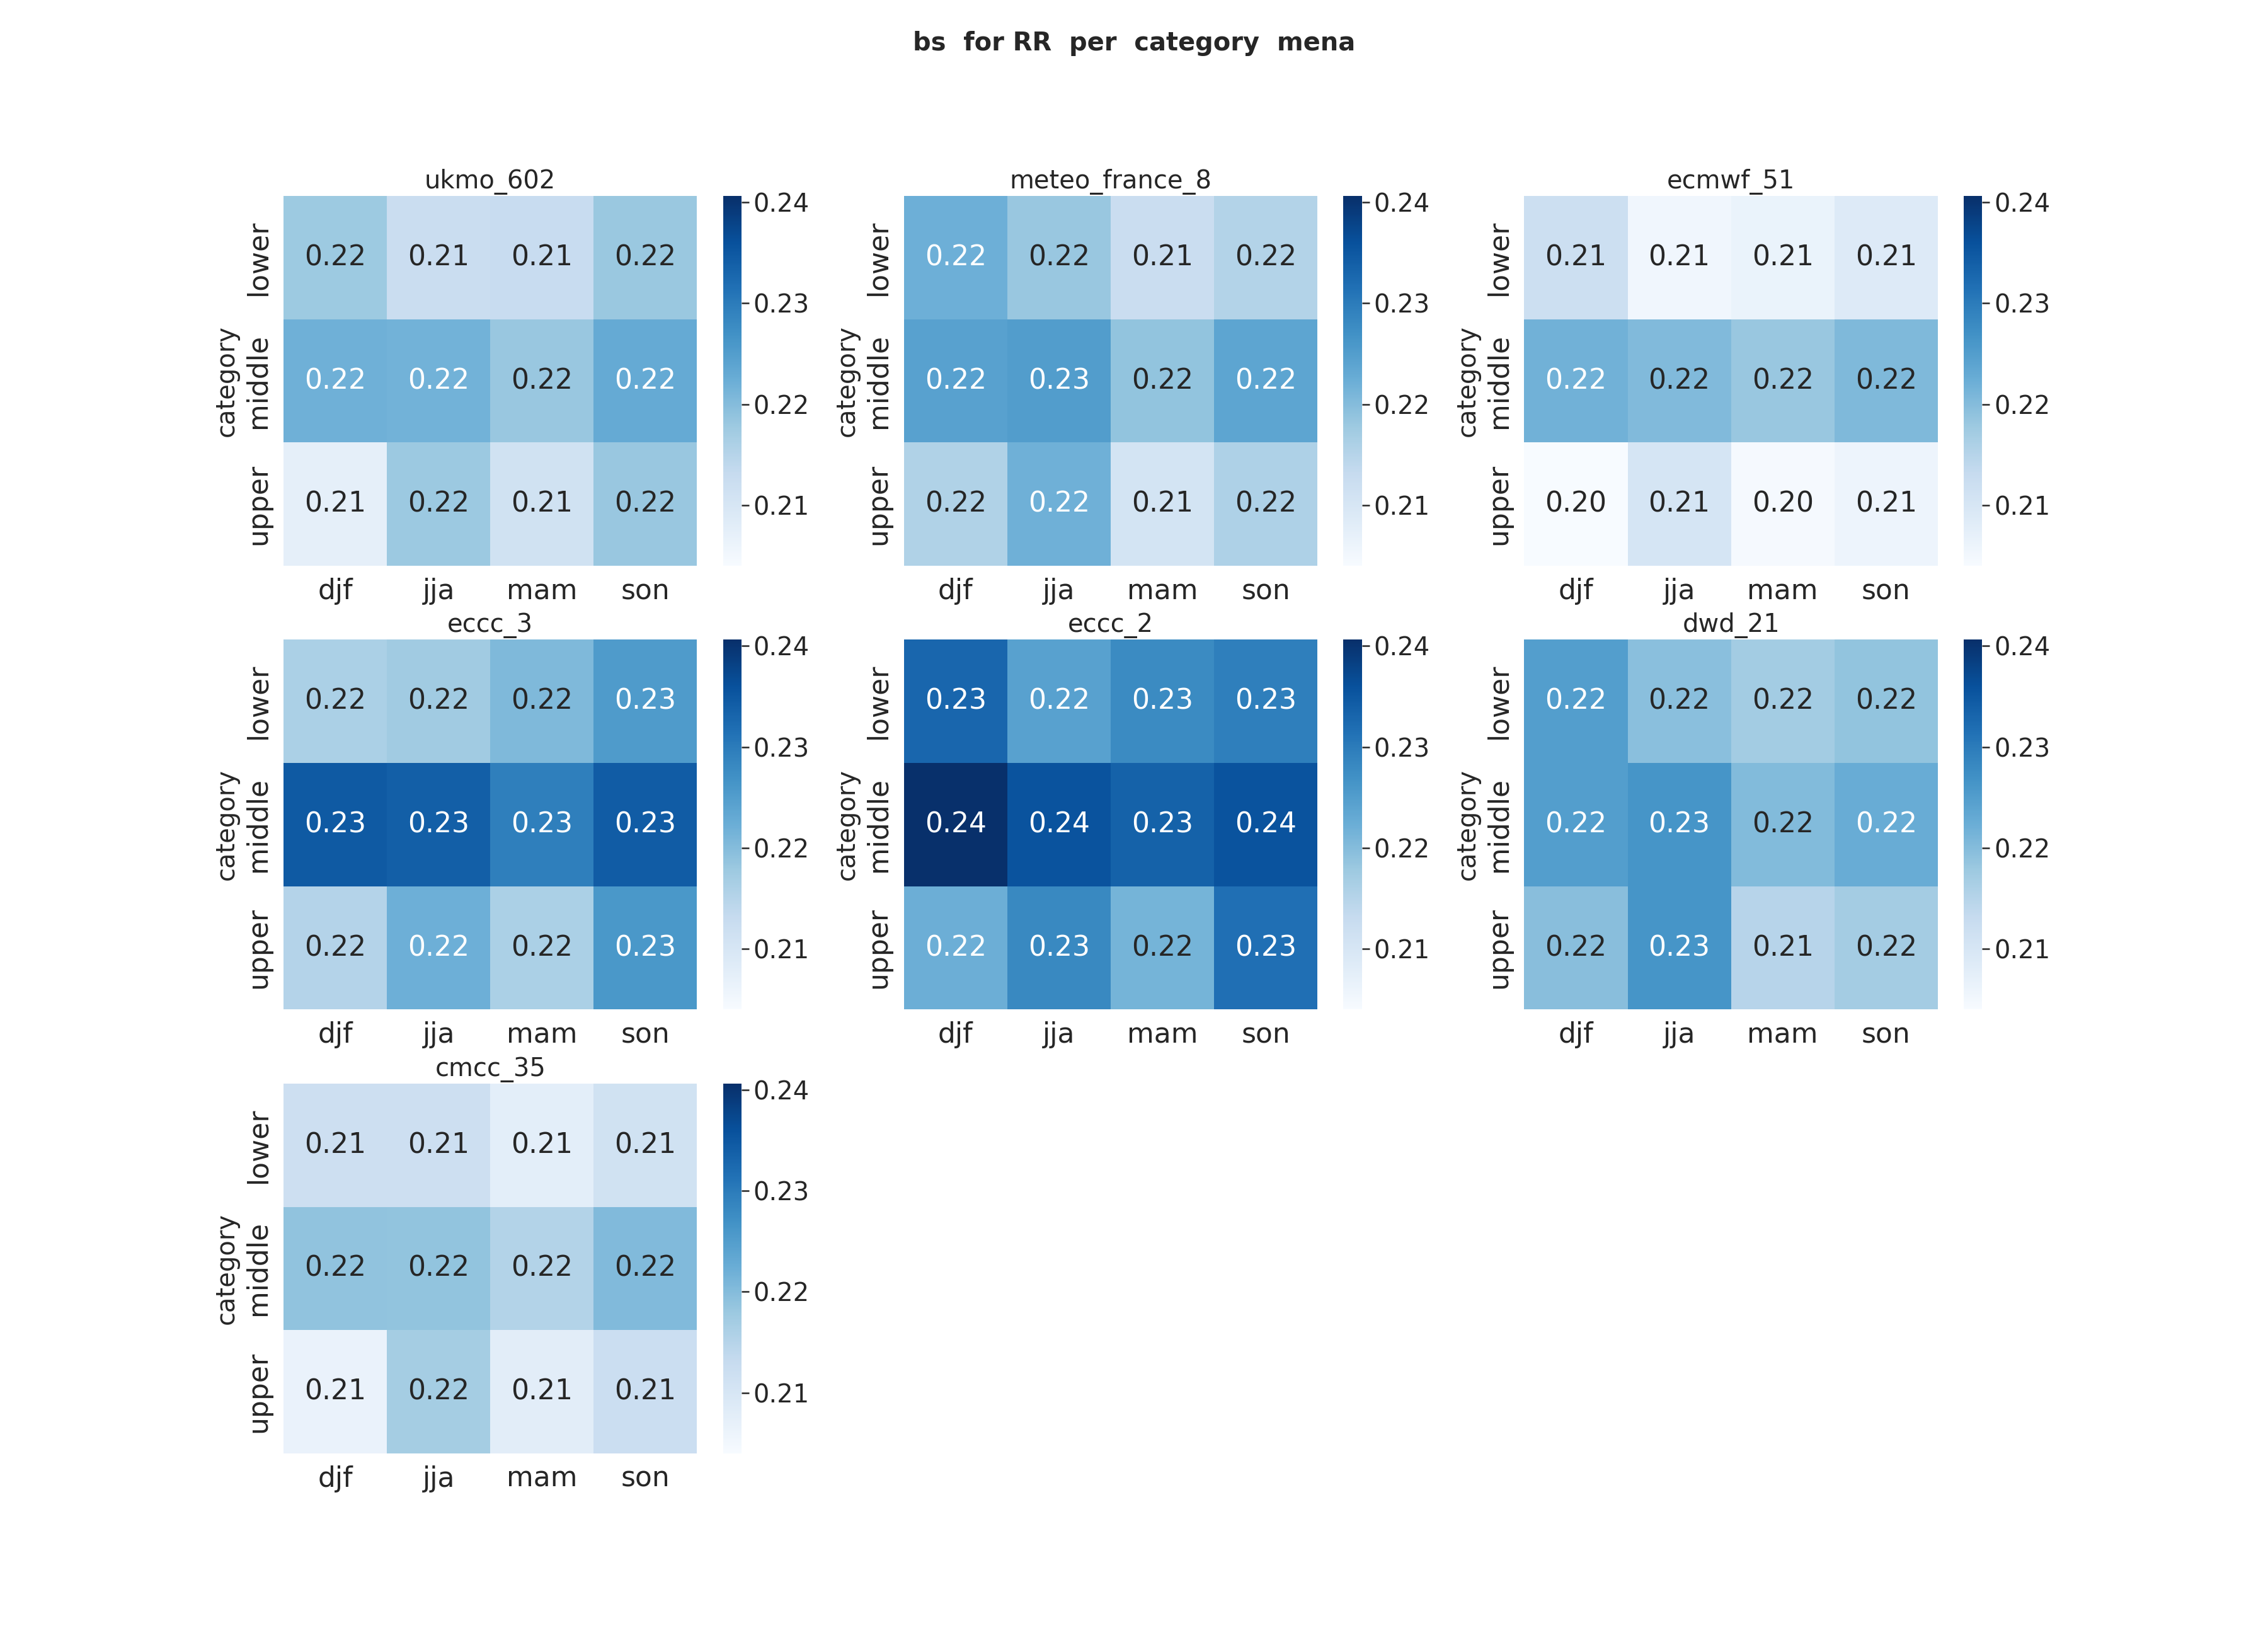
\includegraphics[width=0.8\linewidth]{/home/mohamed/EHTPIII/MODELISATION/Report_25_11/plots/prob/bs/bs_RR_category_mena.png}
    \caption{Heatmap BS par Catégorie.  }
    \label{fig:enter-label}
\end{figure}
\end{frame}


\begin{frame}{Précipitation}
\framesubtitle{Probabiliste - BS (0 pour un BS meilleur)}

\begin{figure}
    \centering
    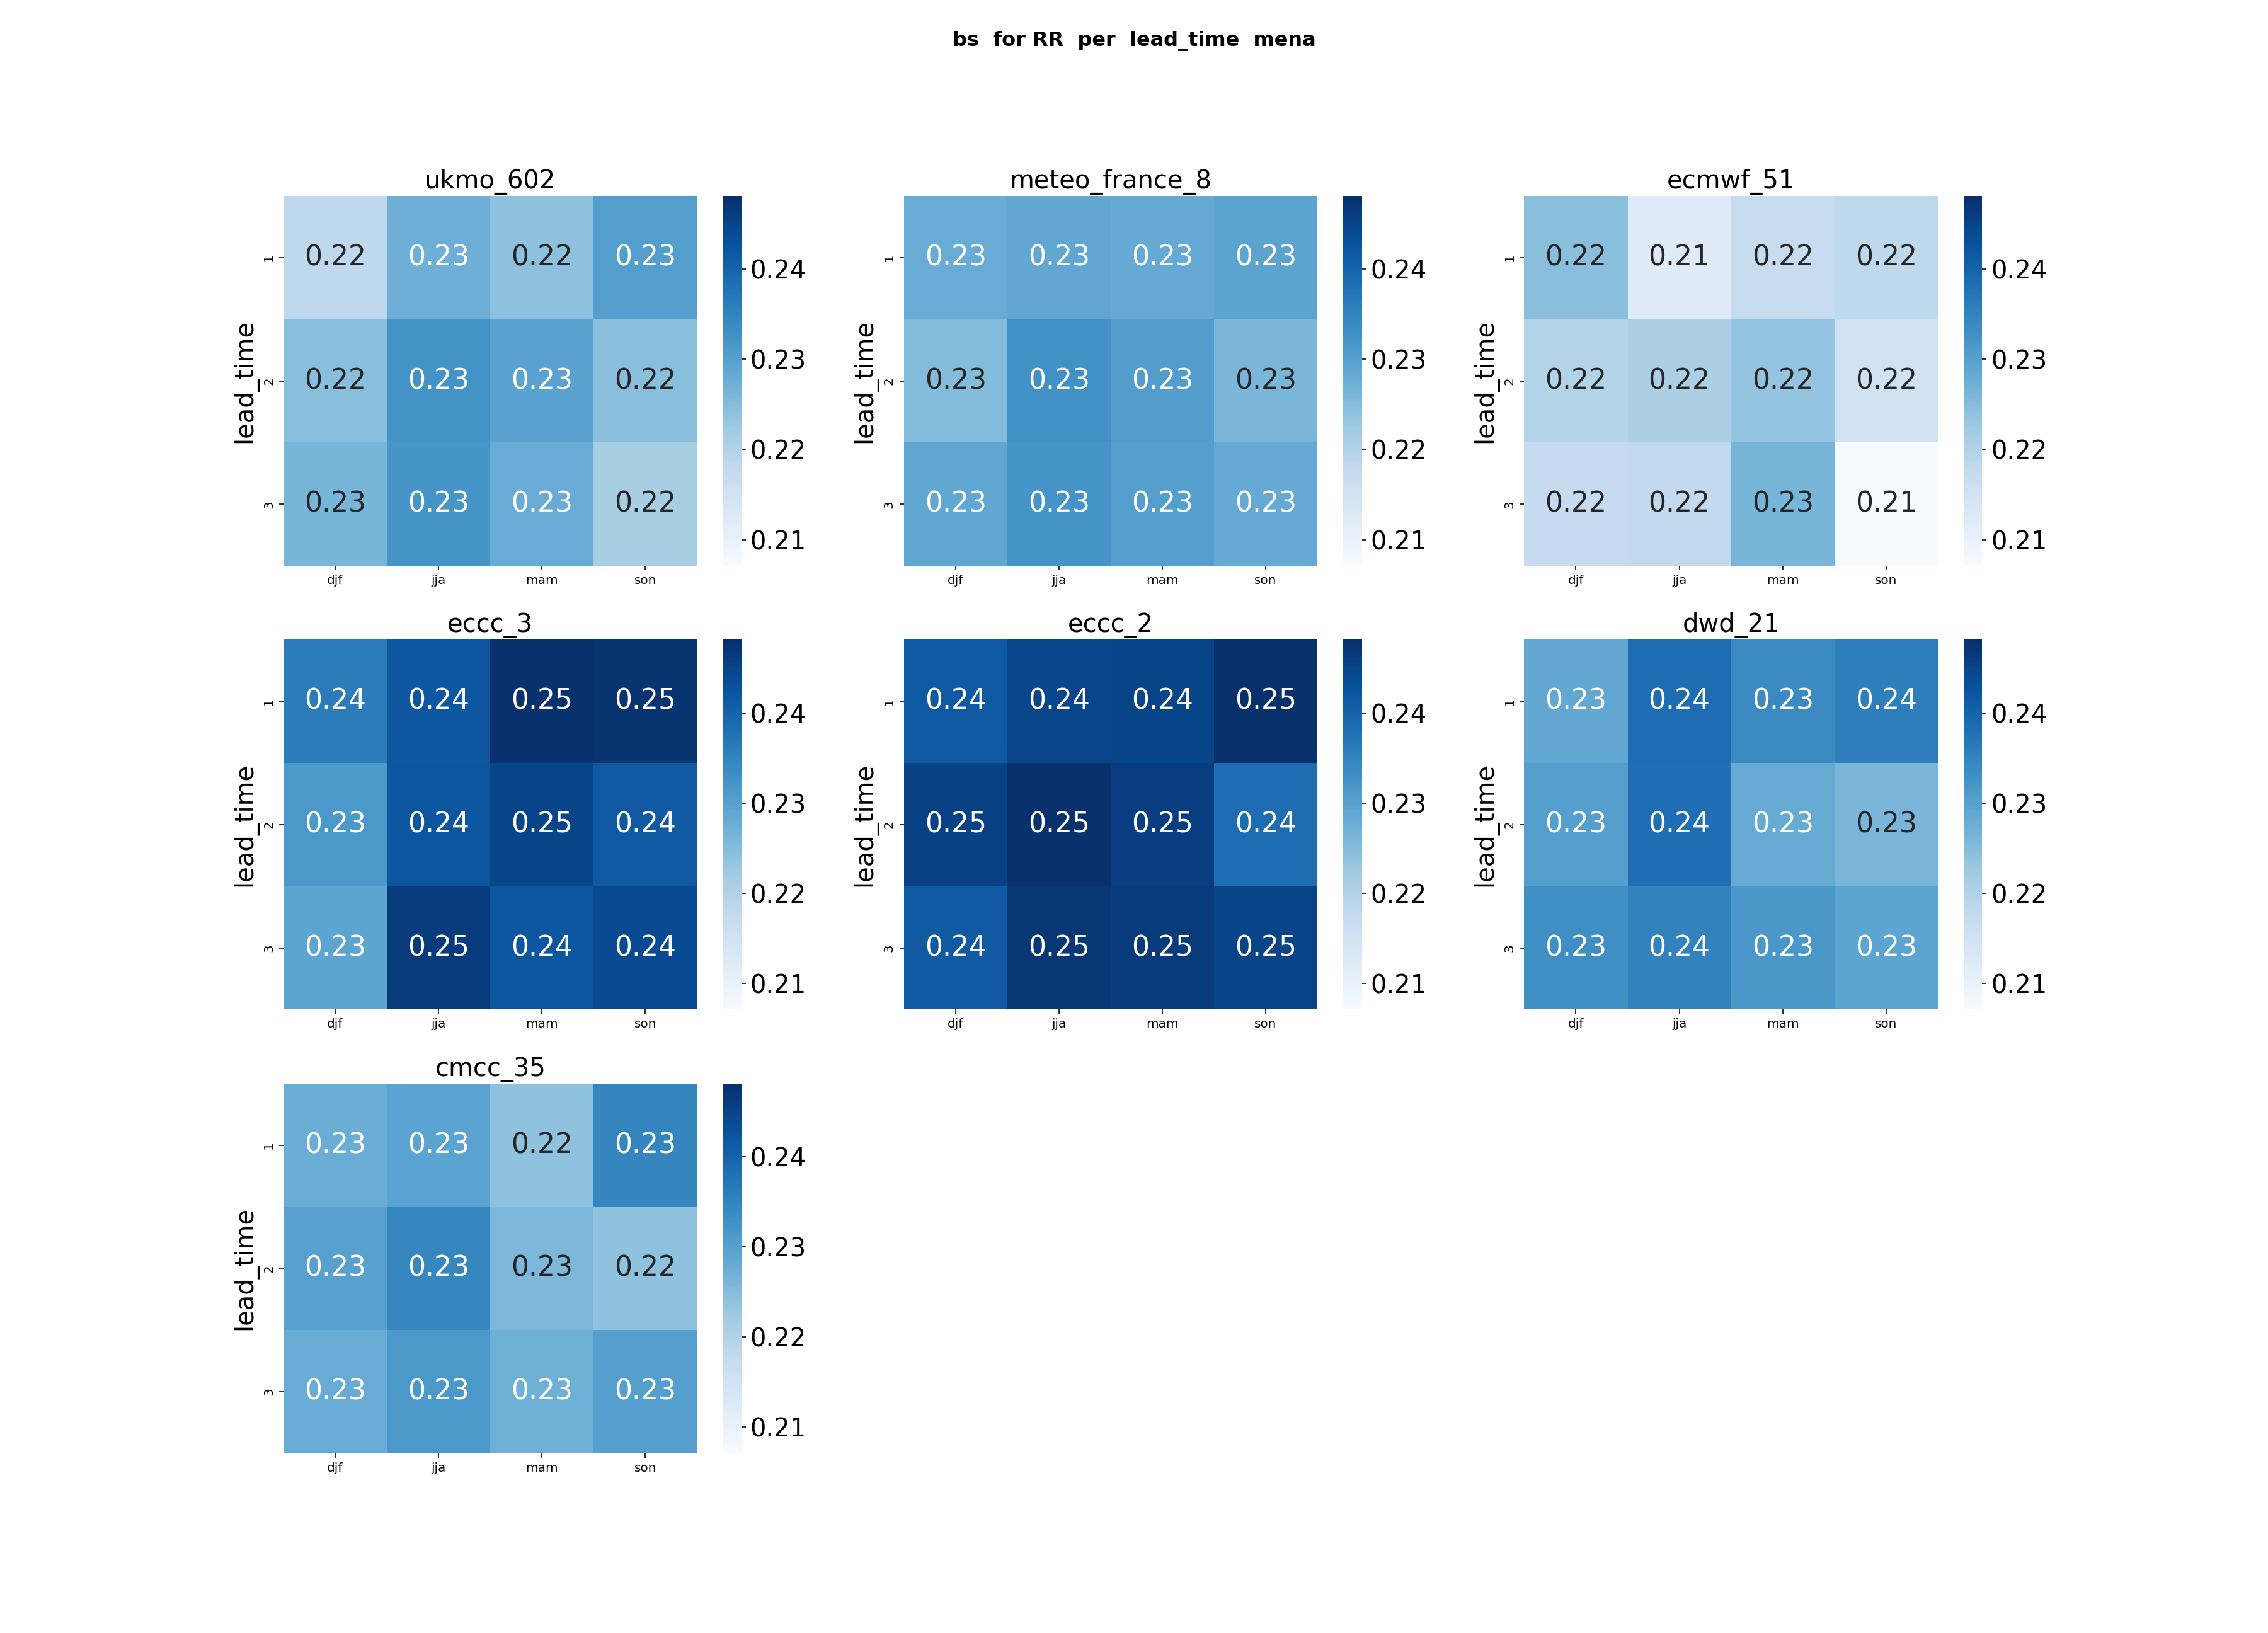
\includegraphics[width=0.8\linewidth]{/home/mohamed/EHTPIII/MODELISATION/Report_25_11/plots/prob/bs/bs_RR_lead_time_mena.png}
    \caption{Heatmap BS par Par échéance.}
    \label{fig:enter-label}
\end{figure}
\end{frame}




\begin{frame}{Précipitation}
\framesubtitle{Probabiliste - ROC (1 pour un ROC meilleur)}

\begin{figure}
    \centering
    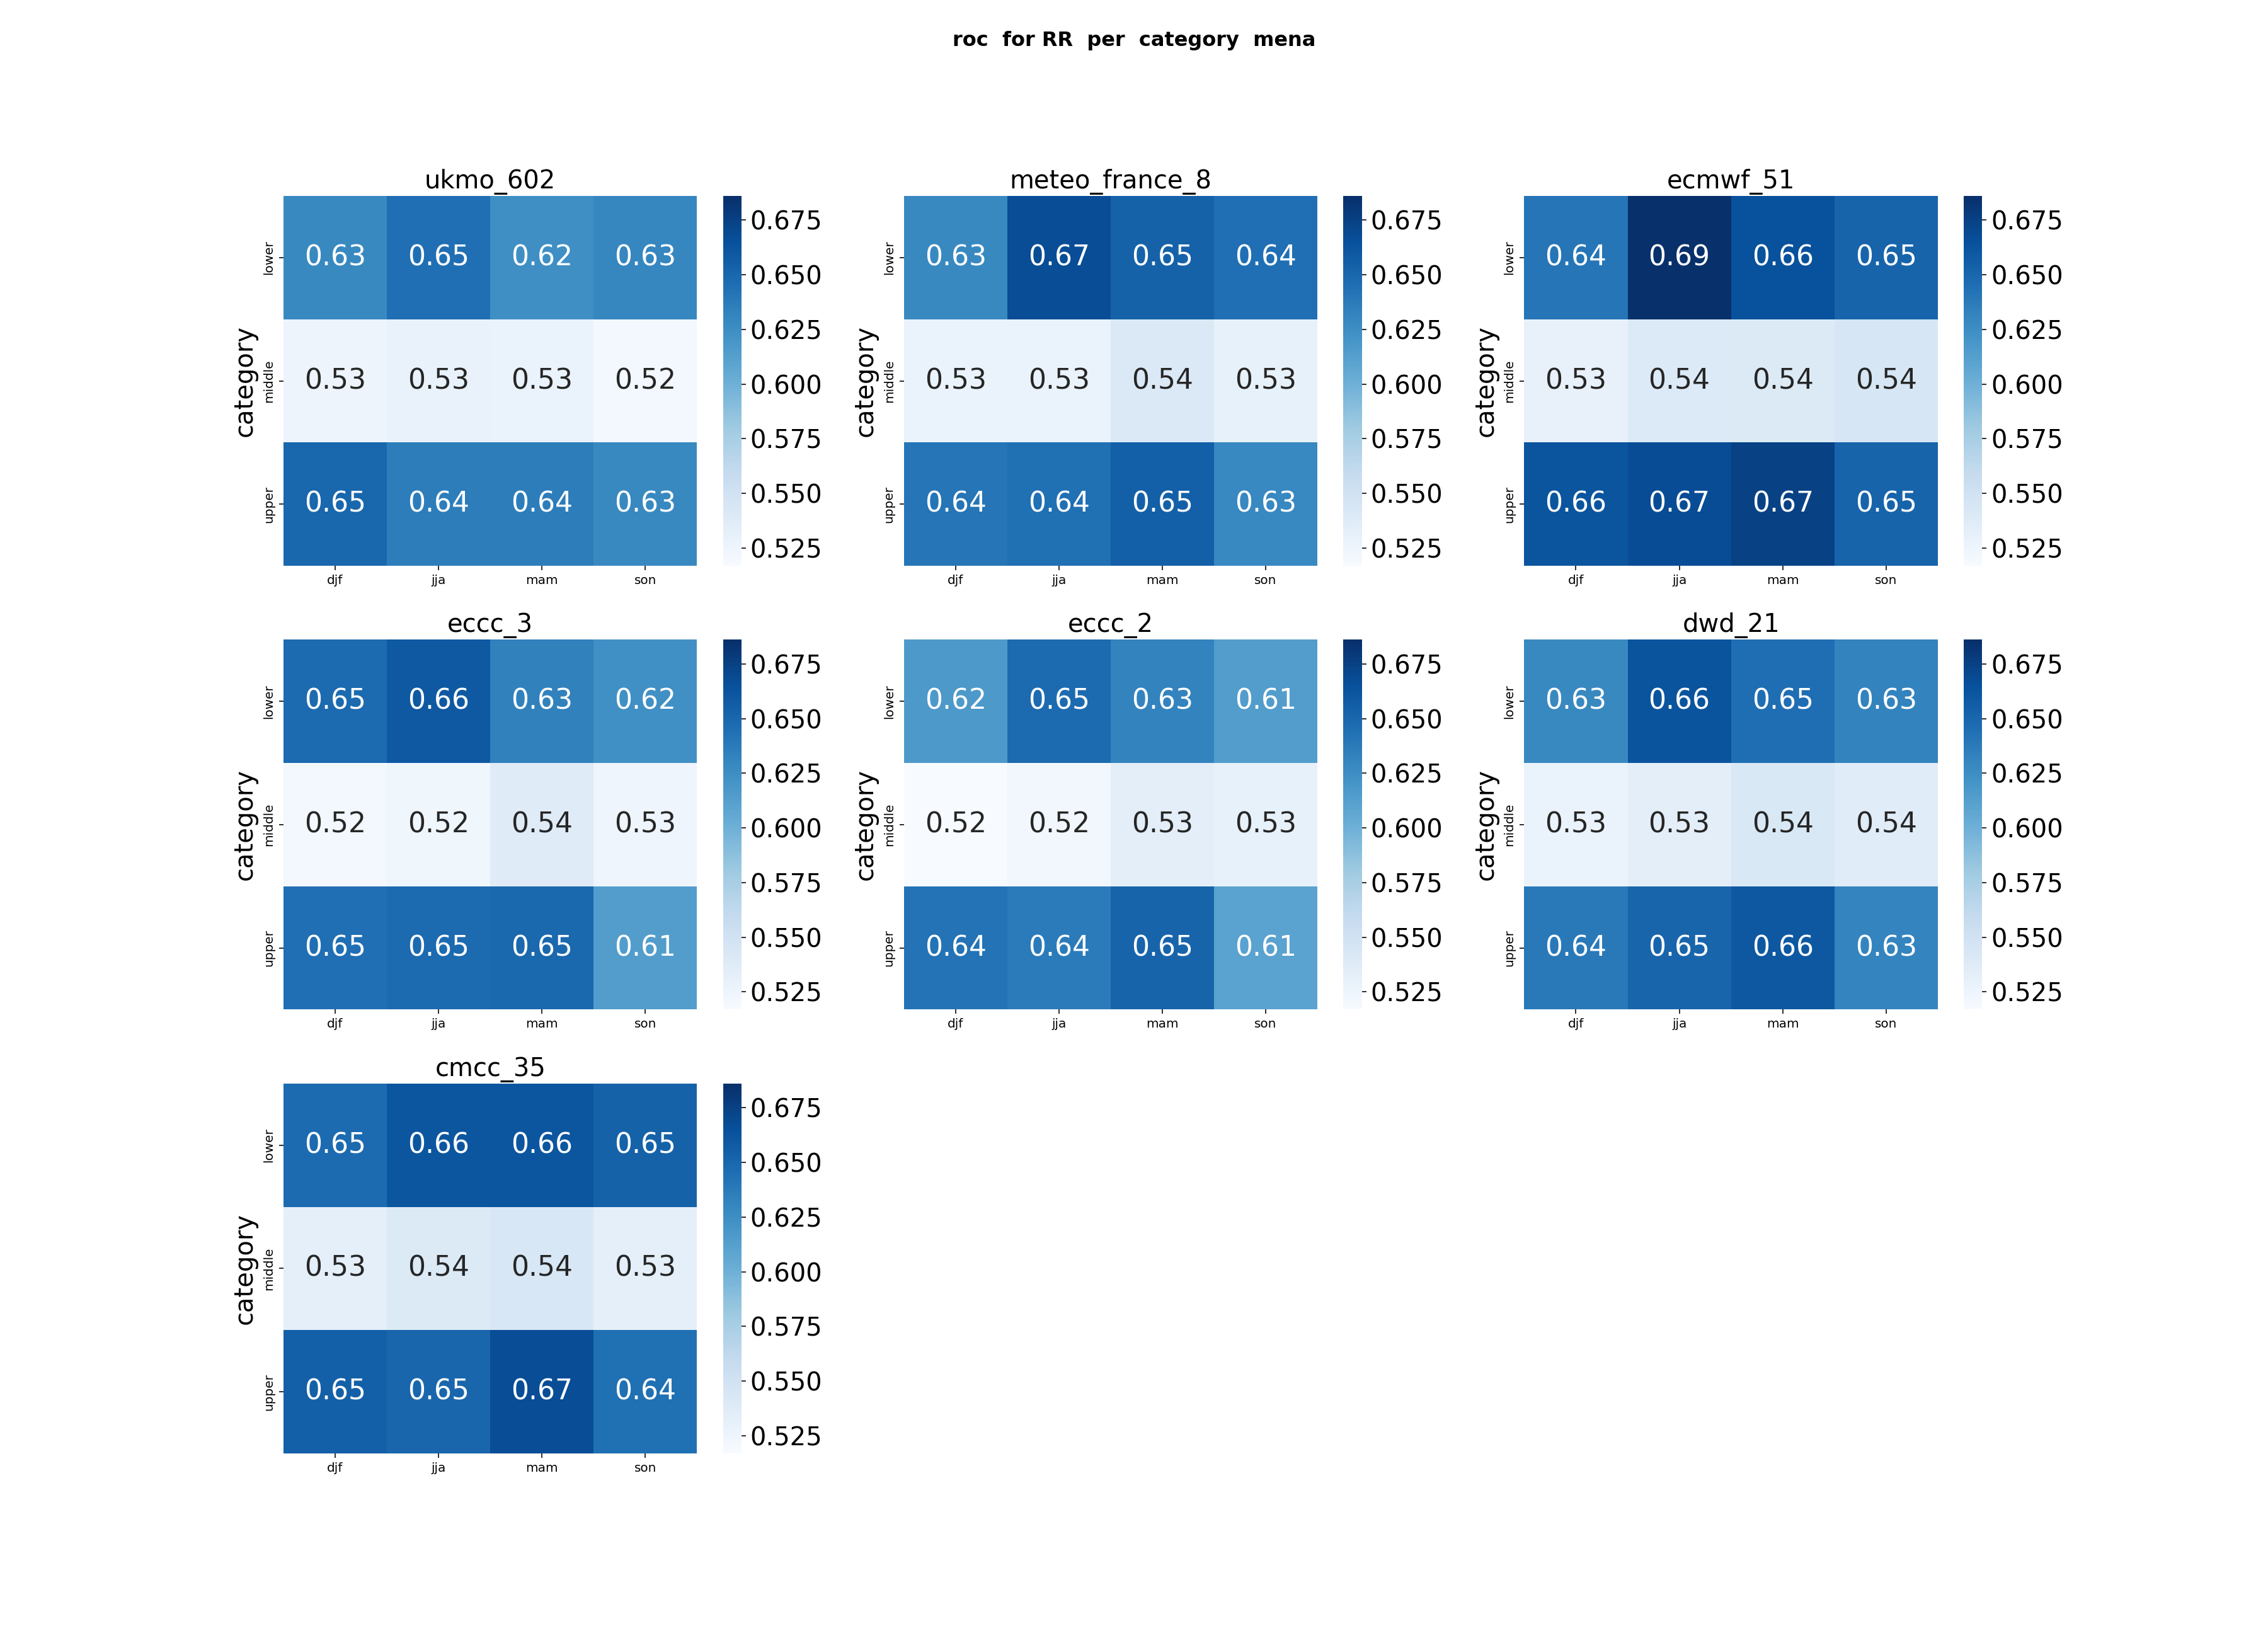
\includegraphics[width=0.8\linewidth]{/home/mohamed/EHTPIII/MODELISATION/Report_25_11/plots/prob/roc/roc_RR_category_mena.png}
    \caption{Heatmap ROC par Catégorie.  }
    \label{fig:enter-label}
\end{figure}
\end{frame}

\begin{frame}{Précipitation}
\framesubtitle{Probabiliste - ROC (1 pour un ROC meilleur)}

\begin{figure}
    \centering
    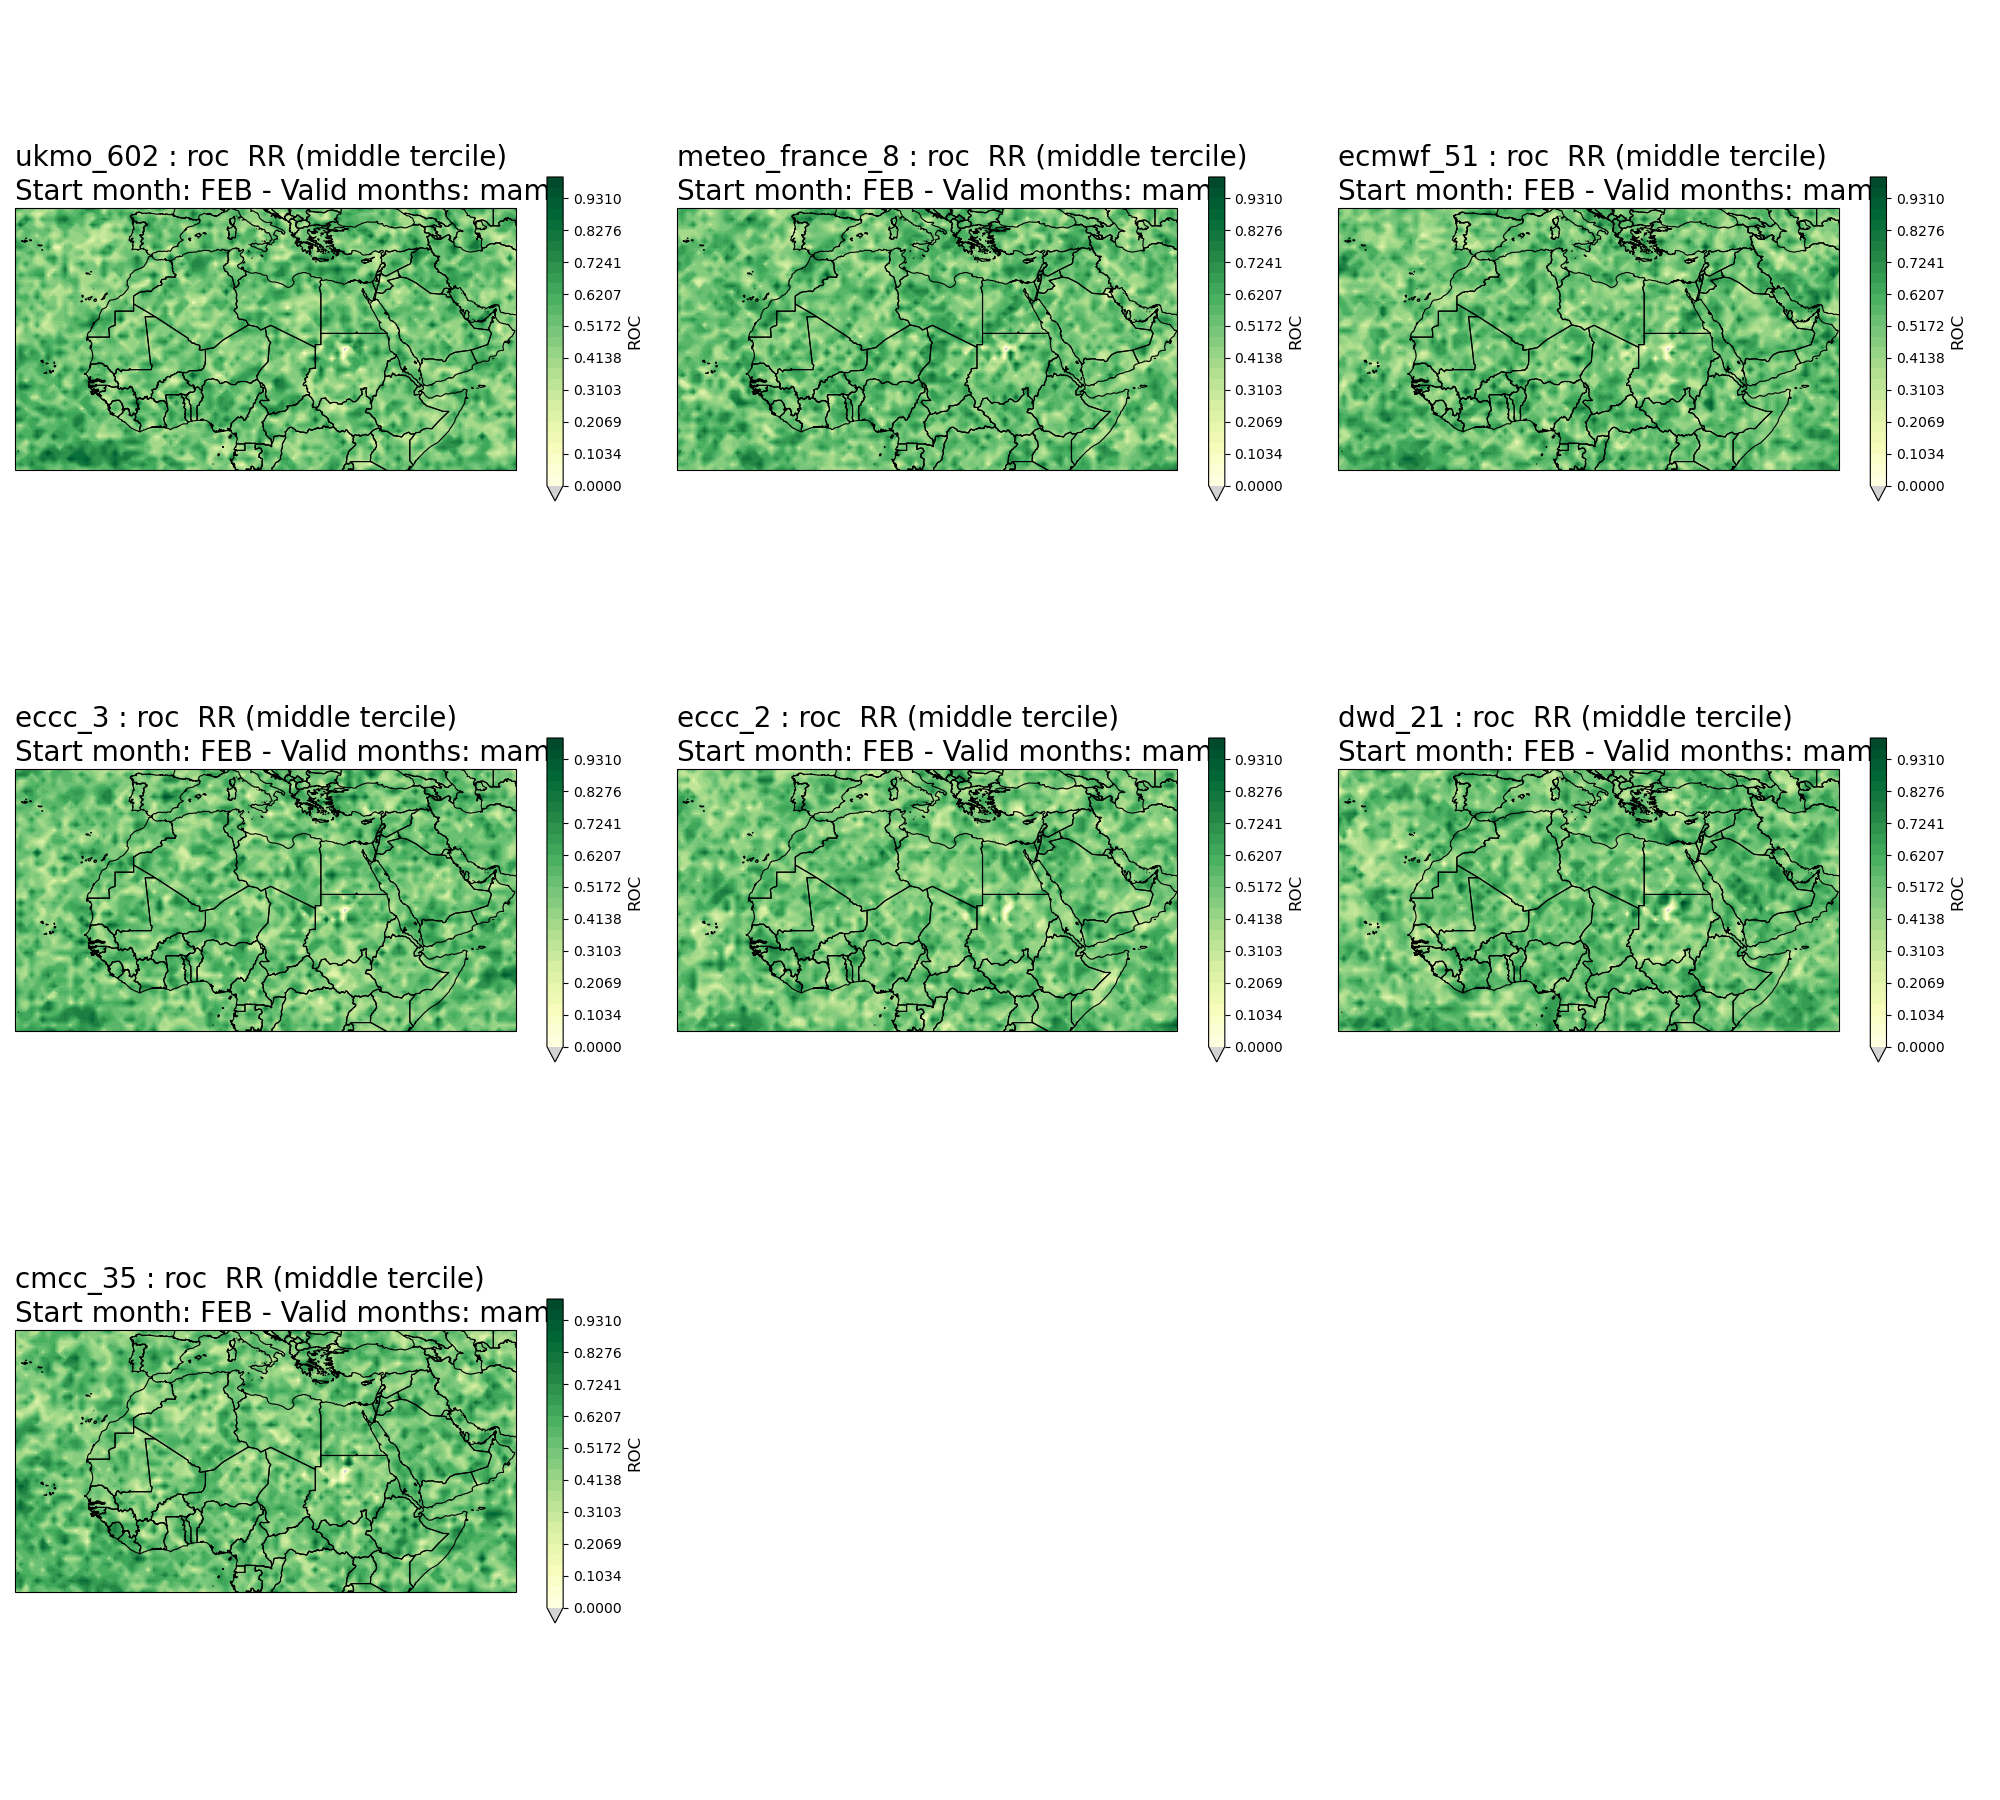
\includegraphics[width=0.7\linewidth]{/home/mohamed/EHTPIII/MODELISATION/Report_25_11/plots/prob/roc/roc_mam_middle_RR.png}
    \caption{ROC pour les Precipitations - MAM  Middle Tercile }
    \label{fig:enter-label}
\end{figure}
\end{frame}


\begin{frame}{Précipitation}
\framesubtitle{Probabiliste - ROC (1 pour un ROC meilleur)}

\begin{figure}
    \centering
    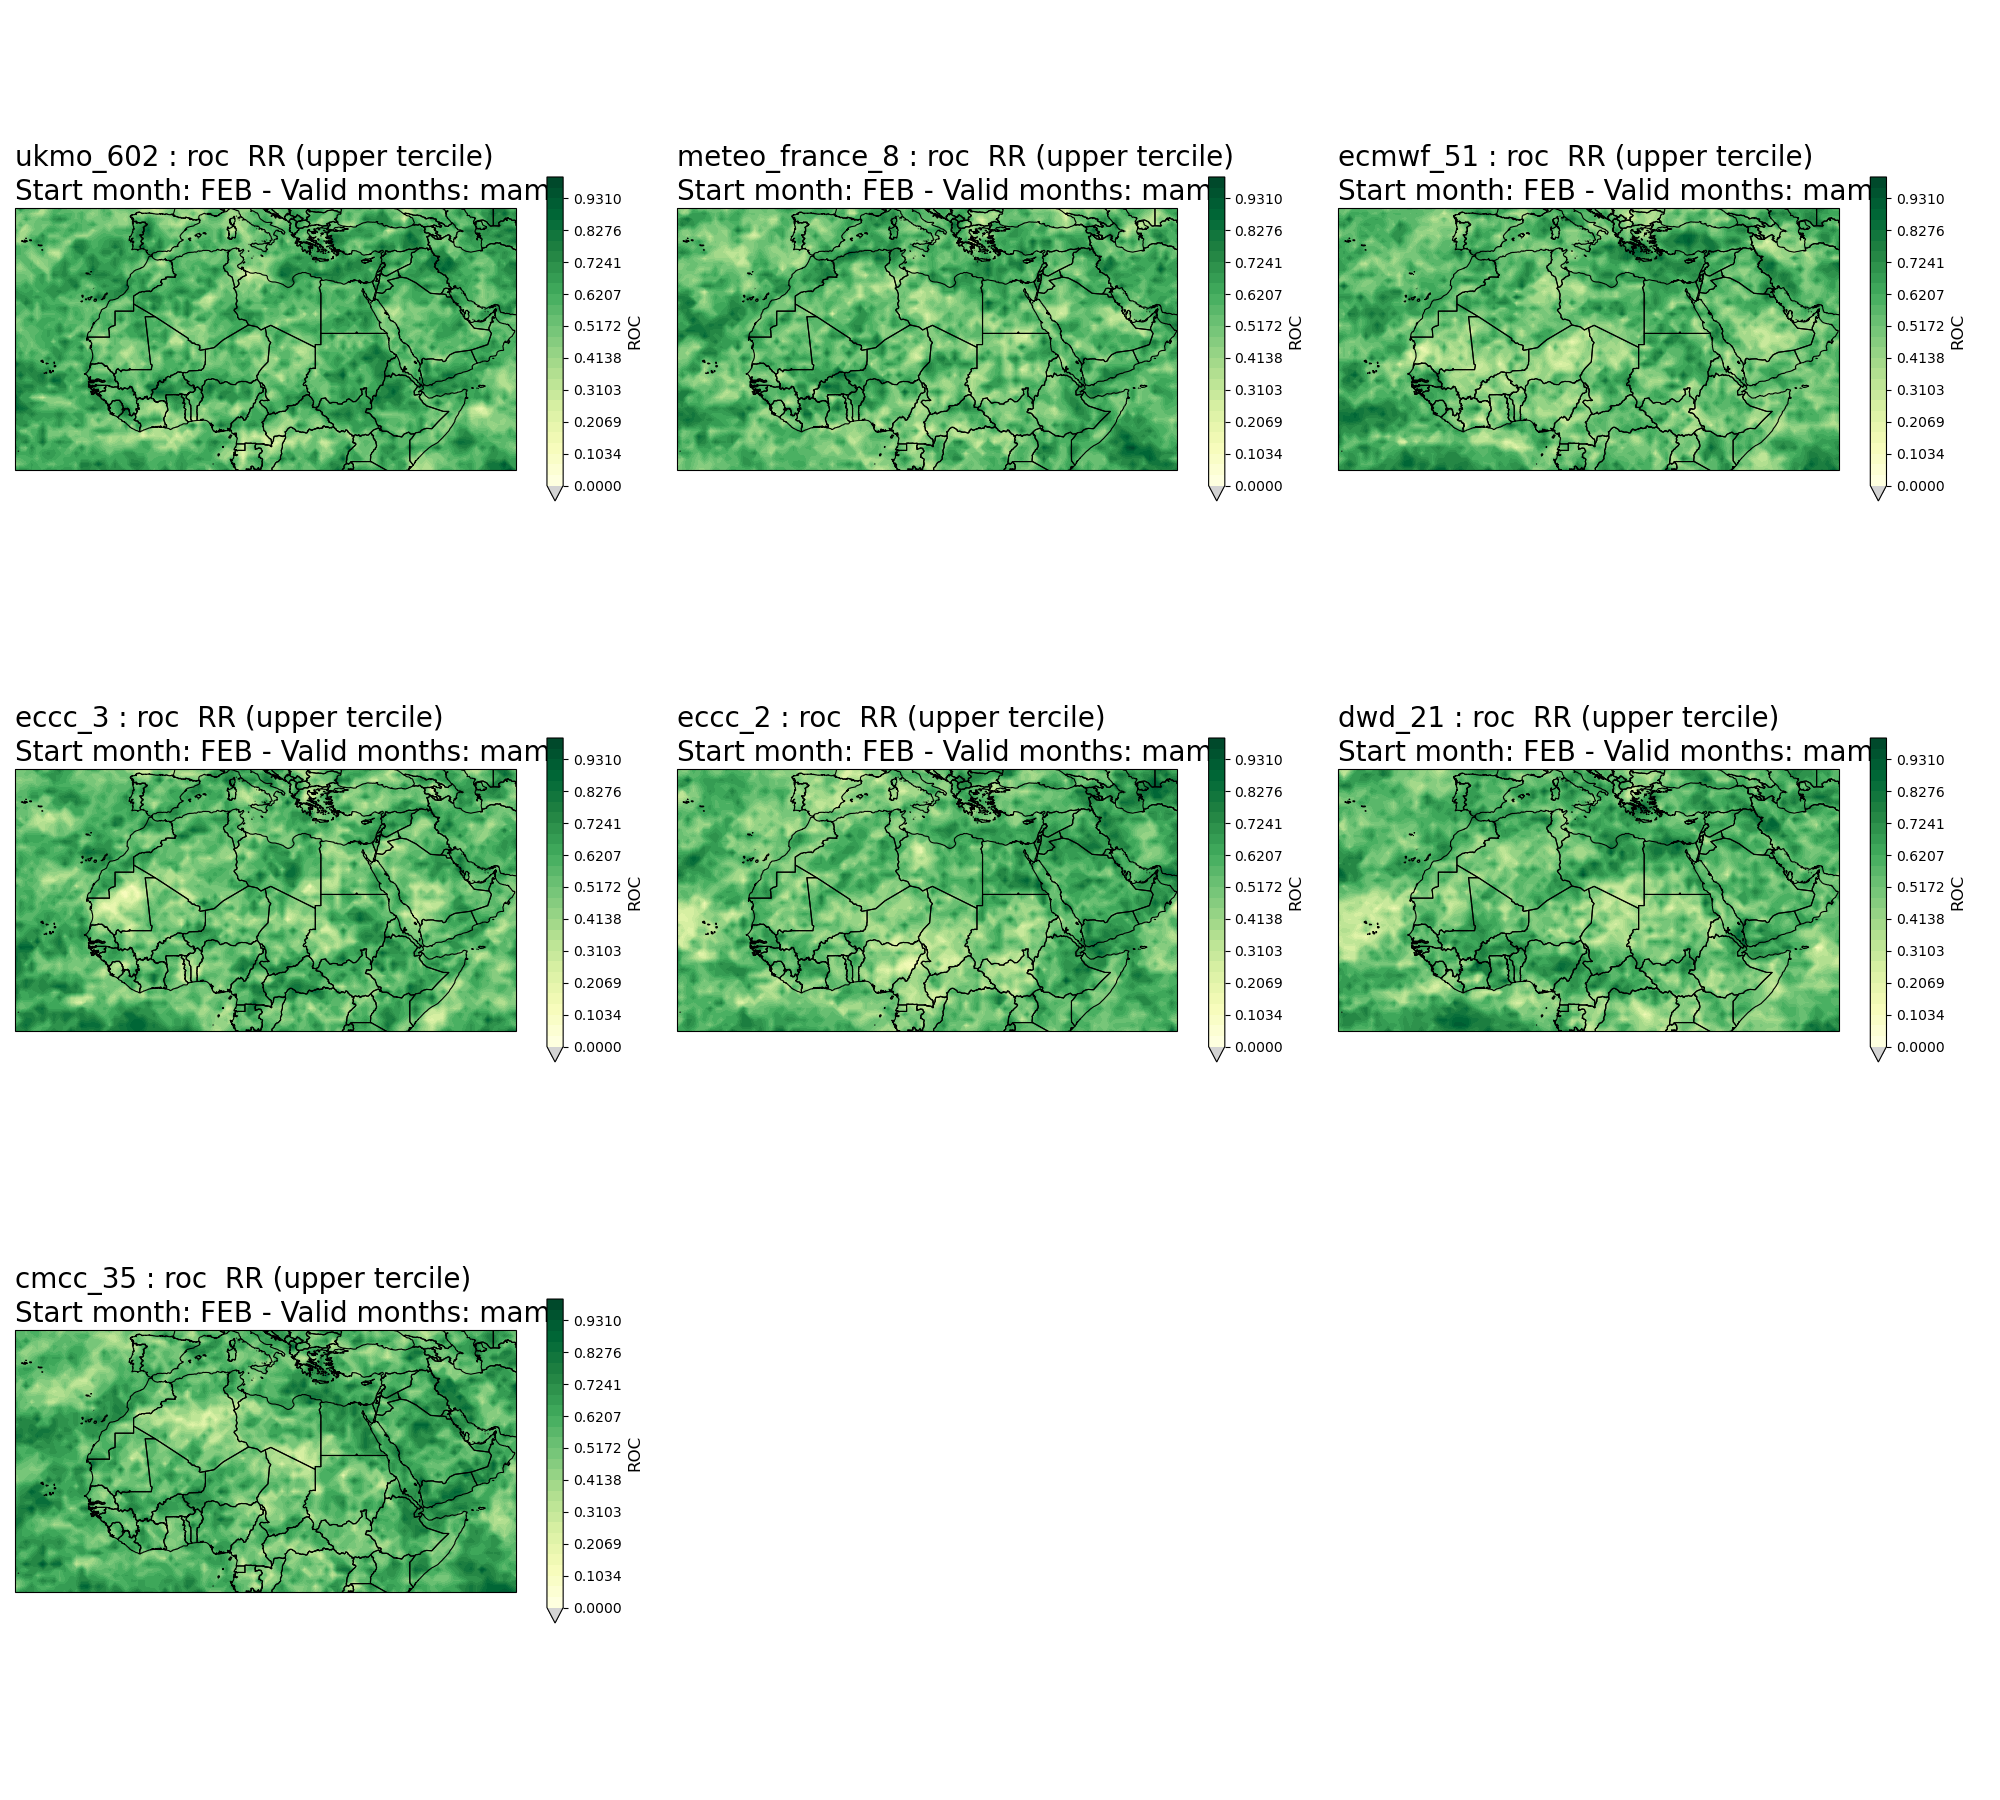
\includegraphics[width=0.7\linewidth]{/home/mohamed/EHTPIII/MODELISATION/Report_25_11/plots/prob/roc/roc_mam_upper_RR.png}
    \caption{ROC pour les Precipitations - MAM  Upper Tercile }
    \label{fig:enter-label}
\end{figure}
\end{frame}



\begin{frame}{Précipitation}
\framesubtitle{Probabiliste - ROC (1 pour un ROC meilleur)}

\begin{figure}
    \centering
    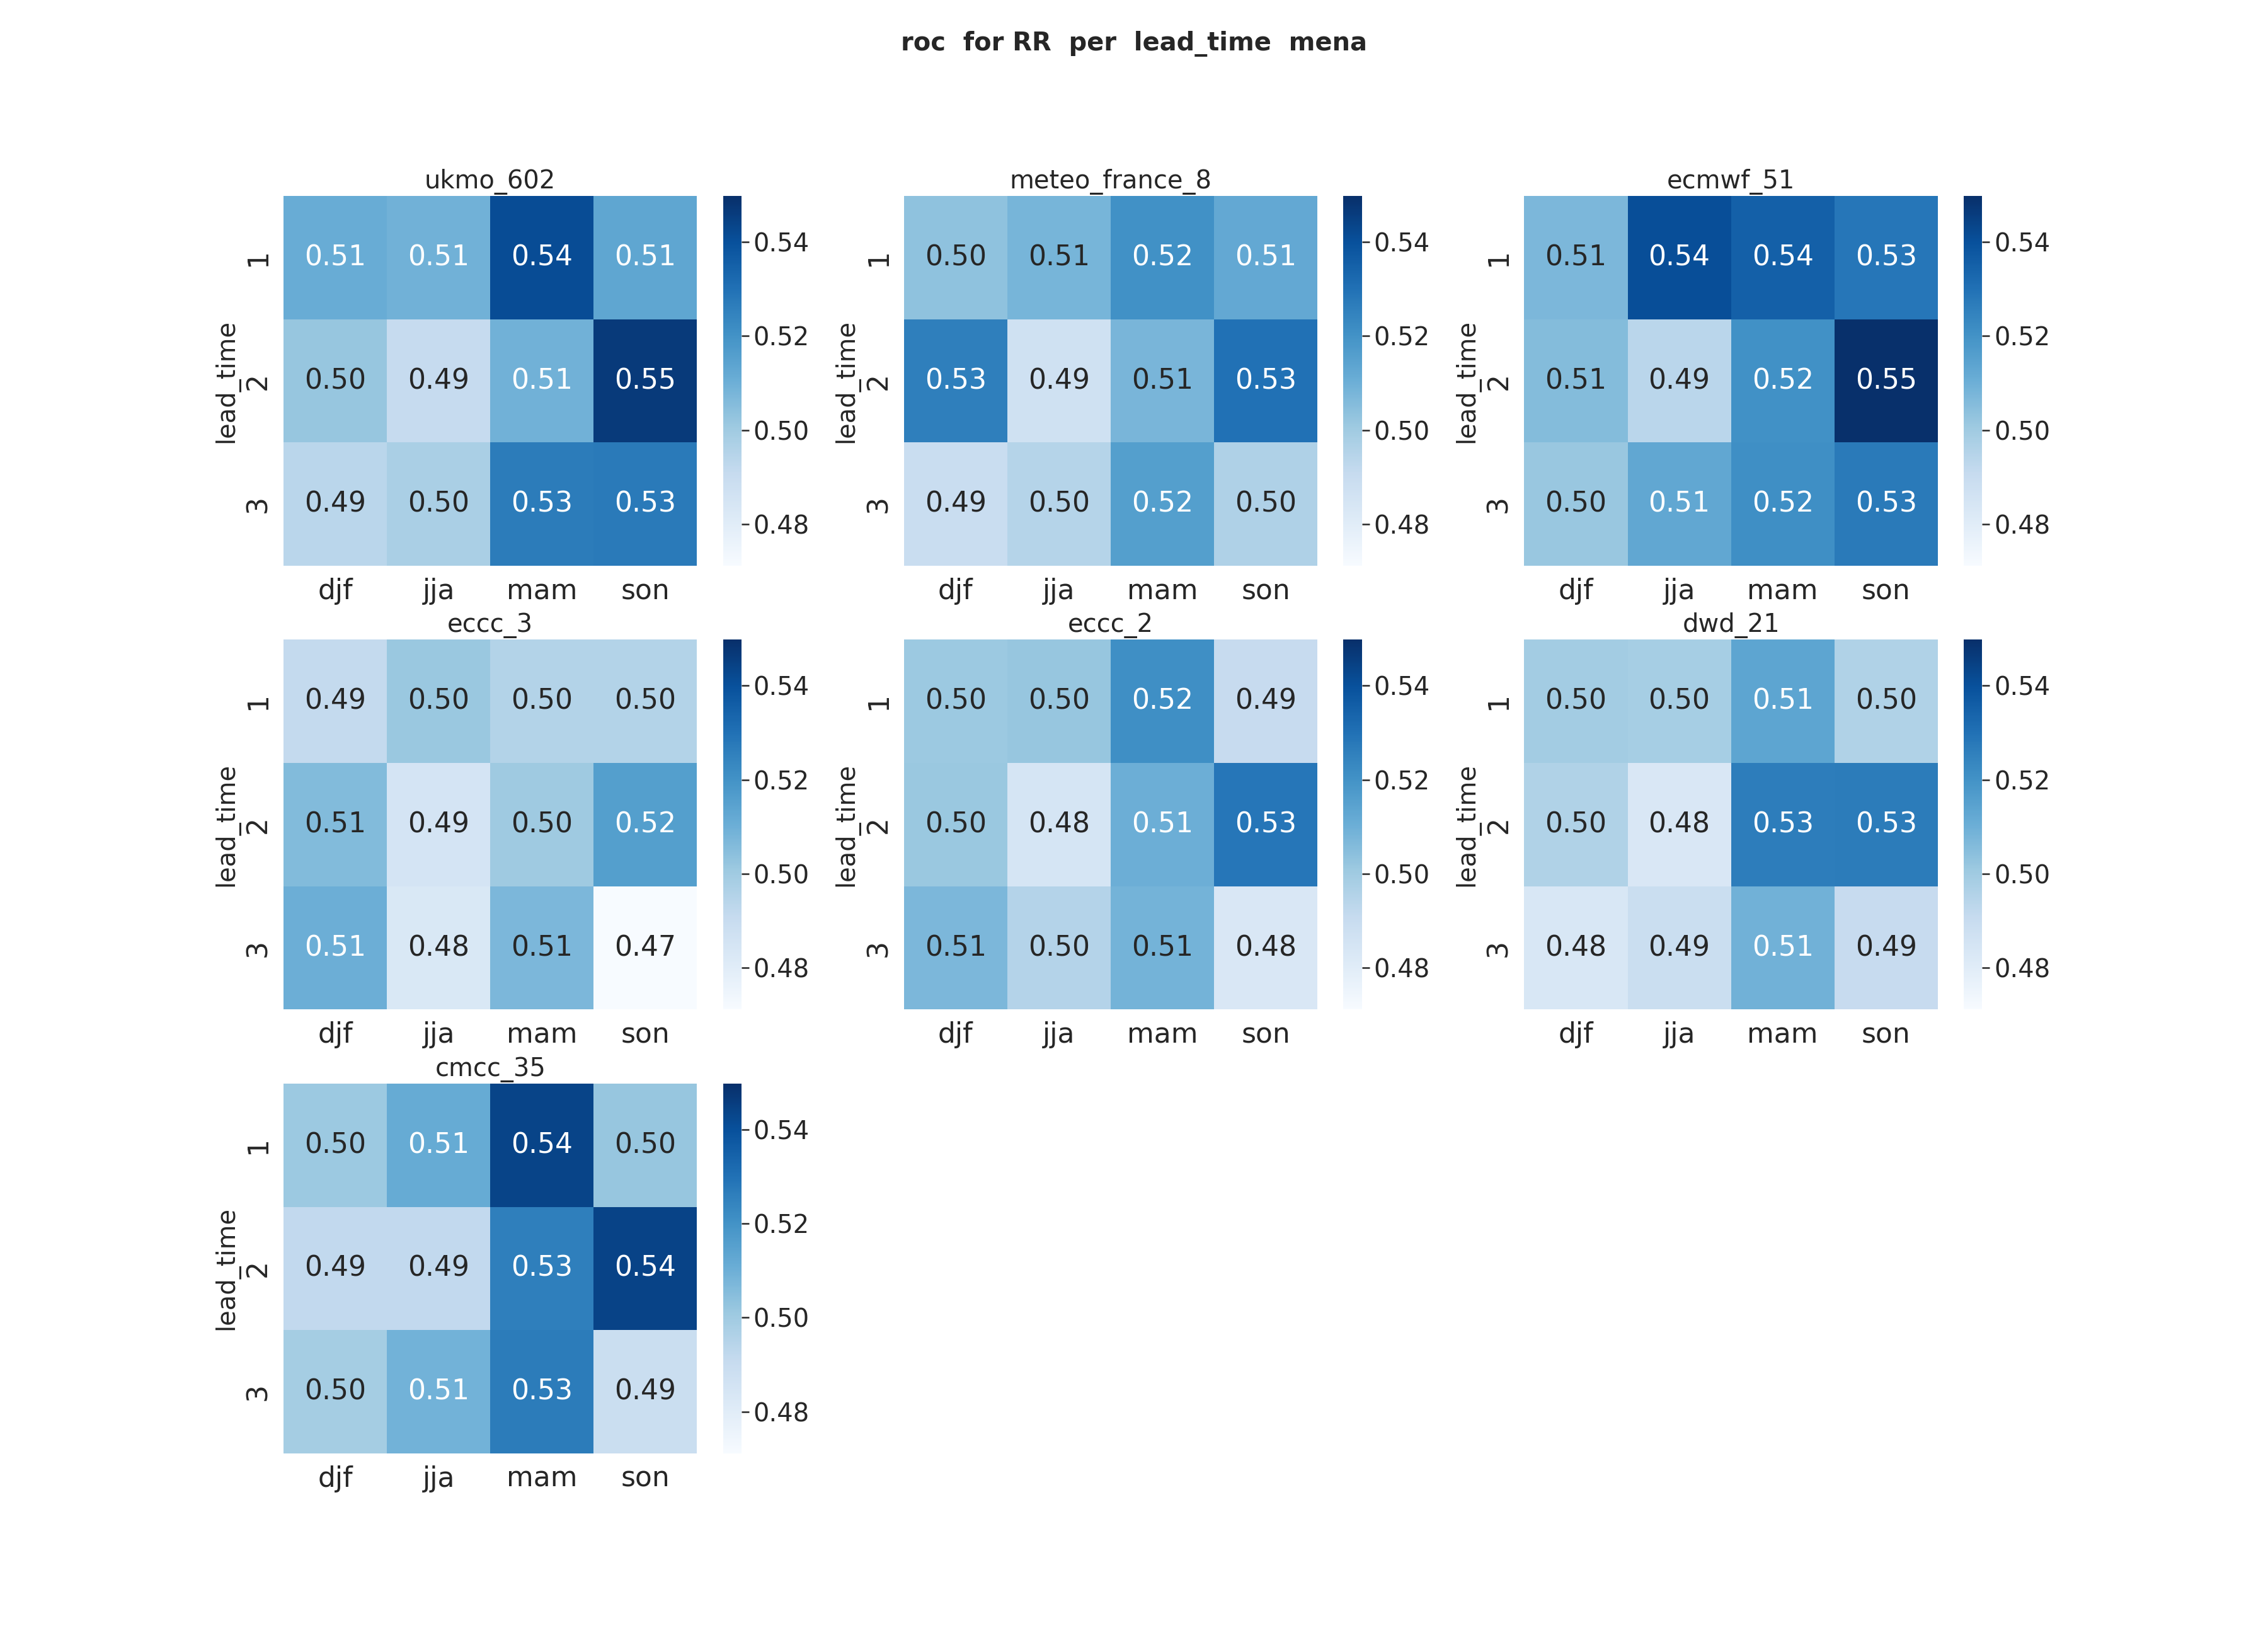
\includegraphics[width=0.8\linewidth]{/home/mohamed/EHTPIII/MODELISATION/Report_25_11/plots/prob/roc/roc_RR_lead_time_mena.png}
    \caption{Heatmap ROC  Par échéance.}
    \label{fig:enter-label}
\end{figure}
\end{frame}

\begin{frame}{Précipitation}
\framesubtitle{Probabiliste - Reliability (45 ° pour un score meilleur)}

\begin{figure}
    \centering
    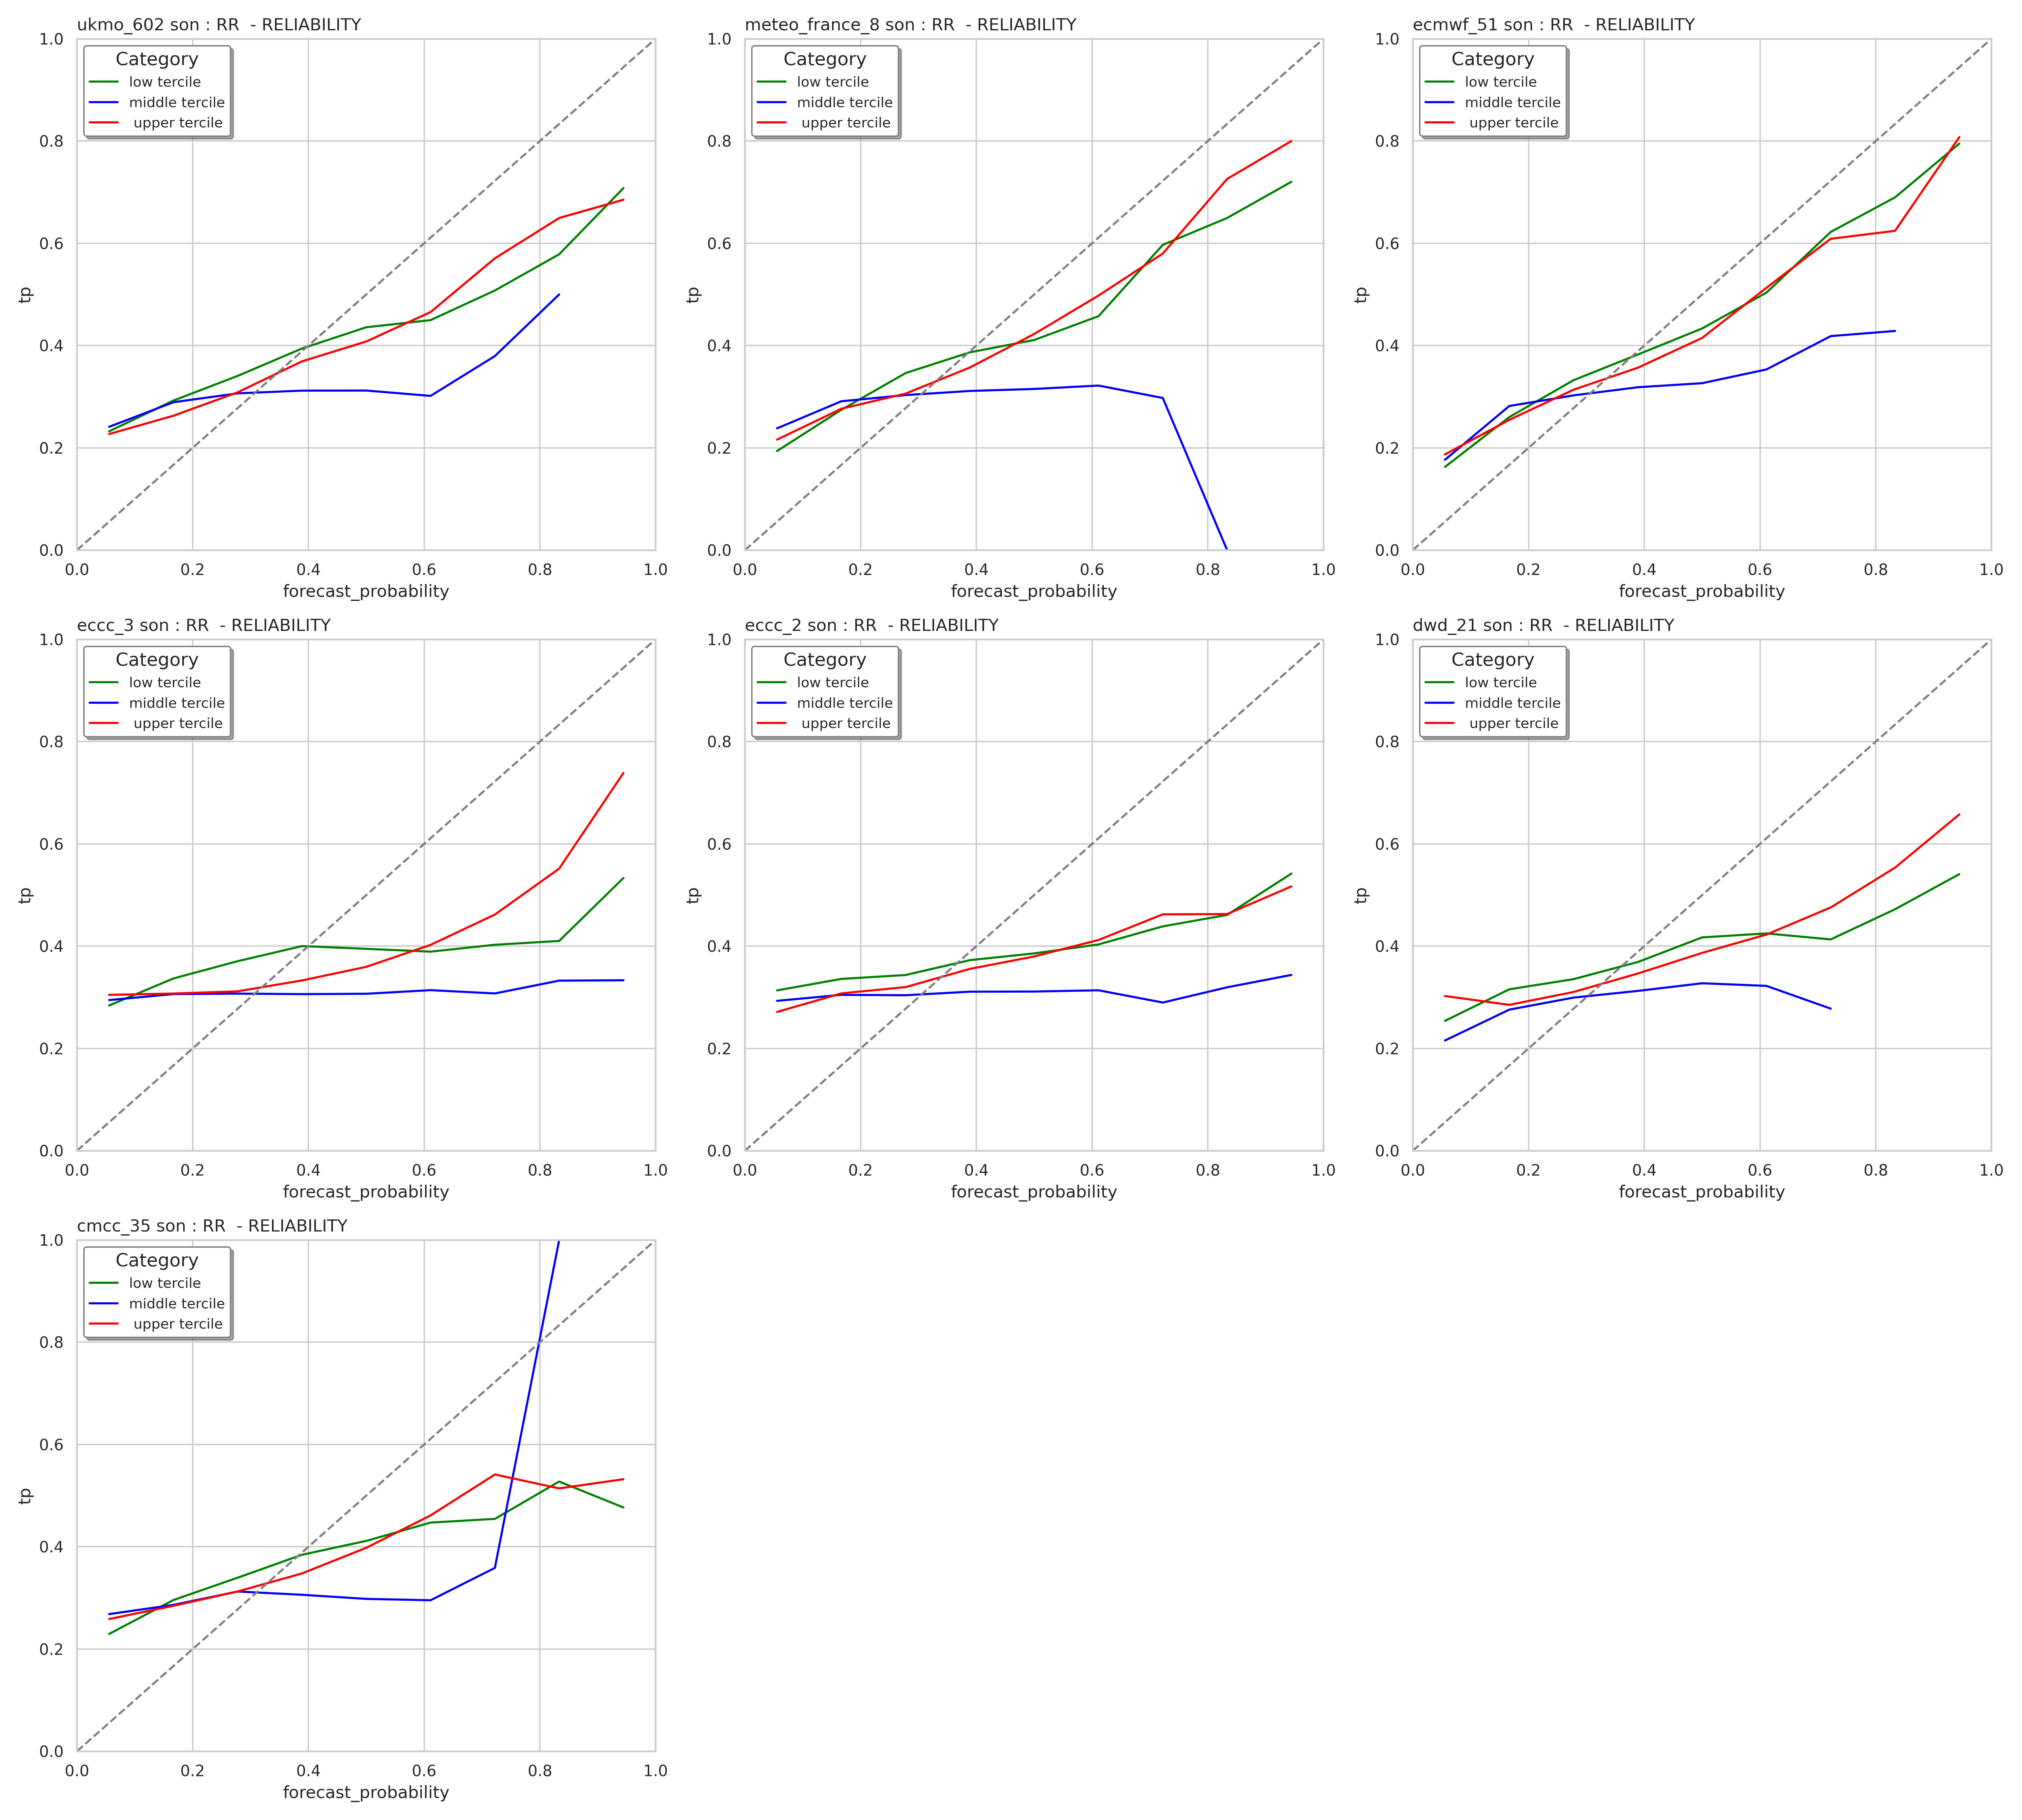
\includegraphics[width=0.6\linewidth]{/home/mohamed/EHTPIII/MODELISATION/Report_25_11/plots/prob/rela/rela_diagram_son_RR.png}
    \caption{Diagramme de Reliability.}
    \label{fig:enter-label}
\end{figure}
\end{frame}

\begin{frame}{CONCLUSION}
\begin{table}[h!]
\centering
\begin{tabular}{|>{\raggedright\arraybackslash}m{1cm}|>{\raggedright\arraybackslash}m{3cm}|>{\raggedright\arraybackslash}m{3cm}|>{\raggedright\arraybackslash}m{3cm}|}
\hline
\textbf{Metric} & \textbf{MENA} & \textbf{North Africa} & \textbf{Arabian Peninsula} \\ \hline
ACC & ECMWF, CMCC-35, UKMO & ECMWF, UKMO and METEO-FRANCE & ECMWF, CMCC-35, UKMO \\ \hline
RMSE & DWD, ECMWF and UKMO & ECMWF, UKMO and DWD & ECMWF, UKMO and DWD \\ \hline
R² & ECMWF & ECMWF & CMCC-35, ECCC2 \\ \hline
BS & ECMWF, METEO-FRANCE and CMCC-35 & ECMWF, METEO-FRANCE and CMCC-35 & ECMWF, METEO-FRANCE and CMCC-35 \\ \hline
RELA & ECMWF, CMCC and UKMO & ECMWF, CMCC-35 and UKMO & METEO-FRANCE, DWD \\ \hline
RPS & ALL  & ALL  & ALL  \\ \hline
ROC & ALL & ALL & ALL \\ \hline
ROCSS & ECMWF & ECMWF & UKMO, CMCC-35 \\ \hline

\end{tabular}
\end{table}
\end{frame}
